\documentclass[11 pt, a4paper]{article}
\usepackage[utf8]{inputenc}
\usepackage[english]{babel} %lingua
\usepackage{textcomp}
\usepackage[a4paper,centering,top=2.5cm,bottom=3.0cm,outer=1.5cm,inner=1.5cm]{geometry}	%%reduce margins
\usepackage{graphicx} %immagini
\usepackage{float} %forza [htb]
\usepackage{listings}
\usepackage{color}

\definecolor{mygreen}{rgb}{0,0.6,0}
\definecolor{mygray}{rgb}{0.5,0.5,0.5}
\definecolor{mymauve}{rgb}{0.58,0,0.82}
\definecolor{myblue}{rgb}{0.44,0.62,0.78}
\definecolor{myglifico}{RGB}{254,194,77}

\usepackage[unicode=true]{hyperref} %indice pdf
\hypersetup{breaklinks=true,
pdfauthor={},
pdftitle={},
colorlinks=true,
citecolor=blue,
urlcolor=blue,
linkcolor=myglifico
}

\author{Glifico}
\date{\today}
\title{User guide}

\begin{document}
\maketitle
\begin{figure}[htb!]
\centering
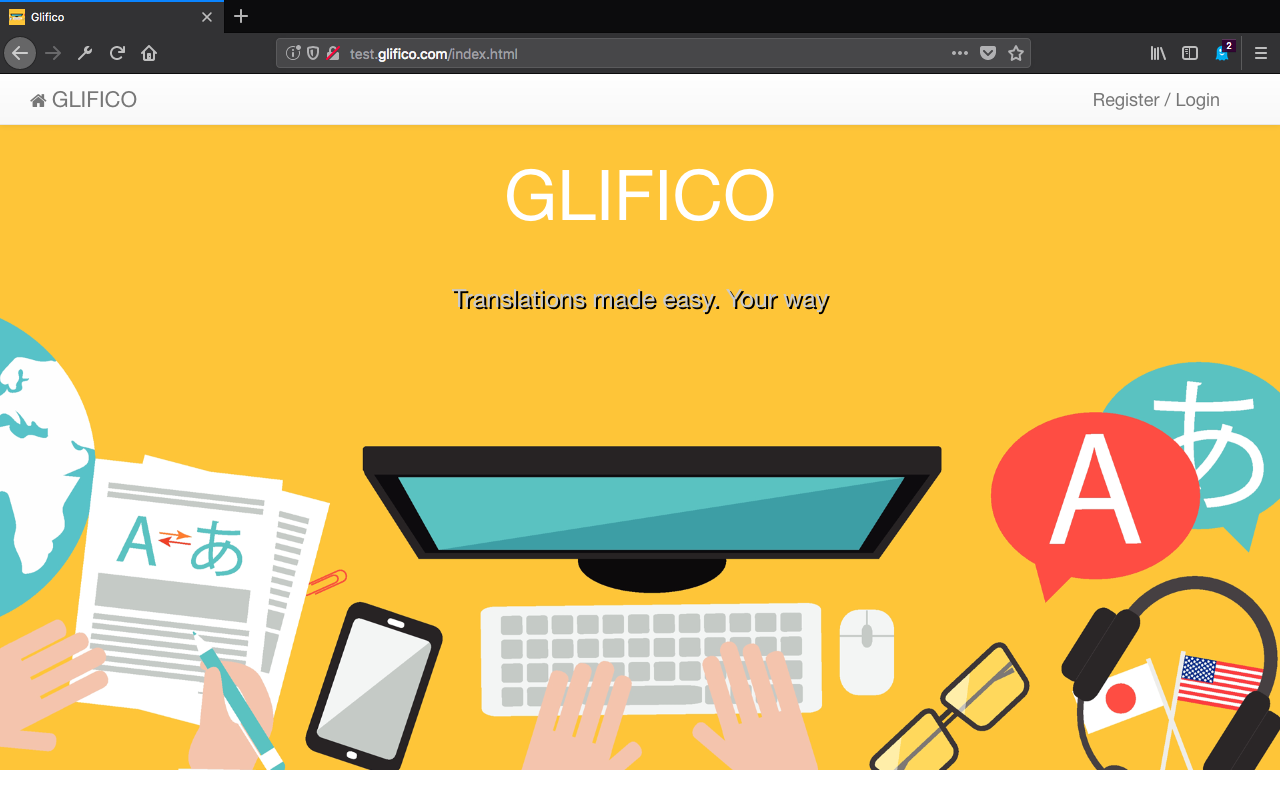
\includegraphics[width=0.95\textwidth]{home.png}
\end{figure}

\newpage
\tableofcontents
\clearpage

\section{Register account}
Follow this steps to register a new account on \url{glifico.com}

Click \textit{Register/Login} on the top left of the page
\begin{figure}[H]
\centering
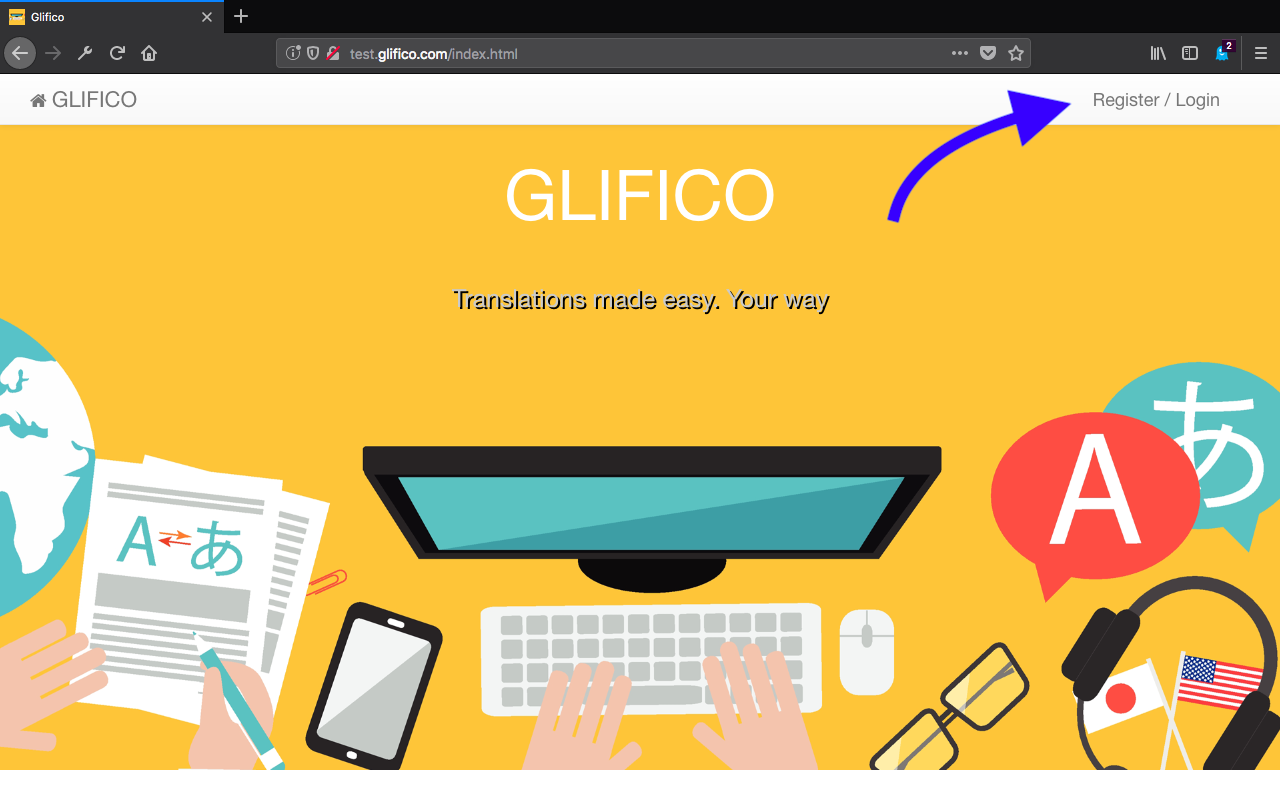
\includegraphics[width=0.95\textwidth]{register_translator0.png}
\end{figure}

Click \textit{Register a new account} and the select \textbf{Translator}
\begin{figure}[H]
\centering
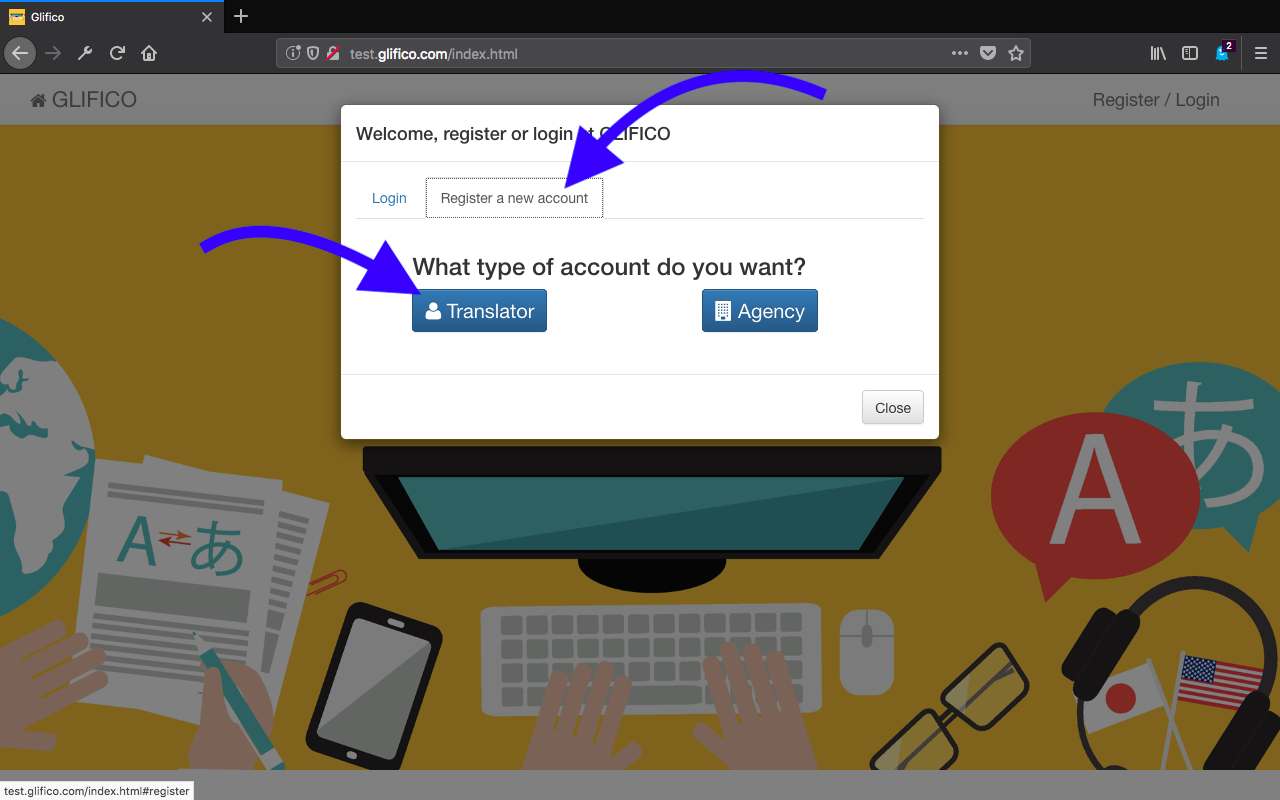
\includegraphics[width=0.95\textwidth]{register_translator1.png}
\end{figure}

\clearpage
Fill the form with all your data
\begin{figure}[H]
\centering
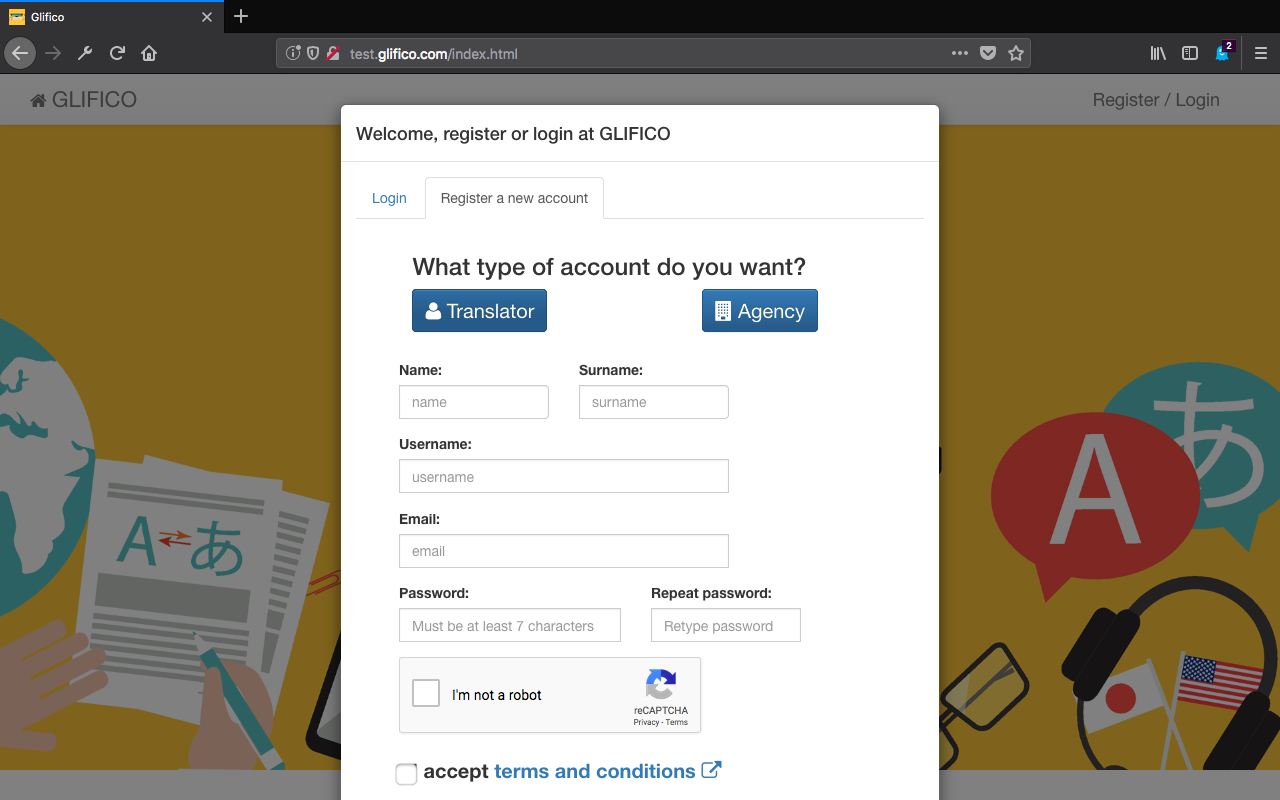
\includegraphics[width=0.95\textwidth]{register_translator2.png}
\end{figure}

\begin{figure}[H]
\centering
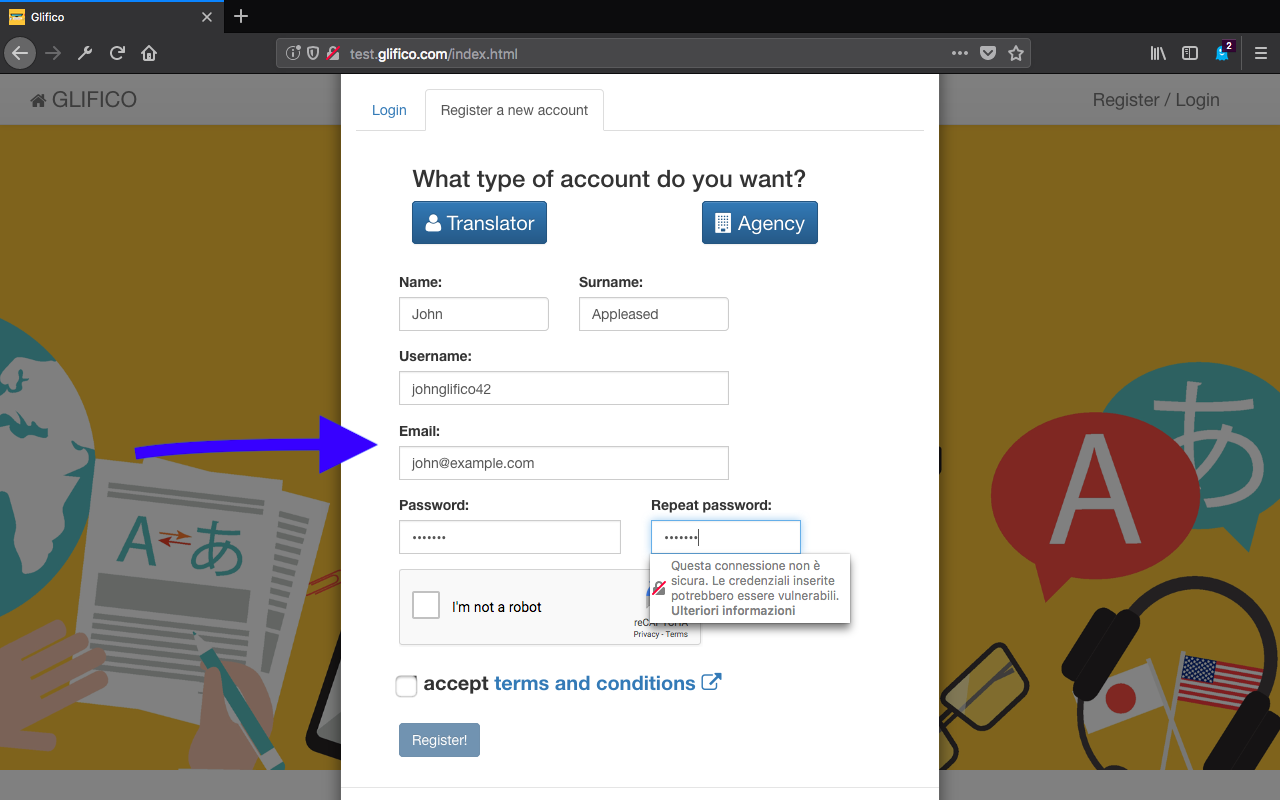
\includegraphics[width=0.95\textwidth]{register_translator3.png}
\end{figure}

\clearpage
Complete the ReCaptcha by Google
\begin{figure}[H]
\centering
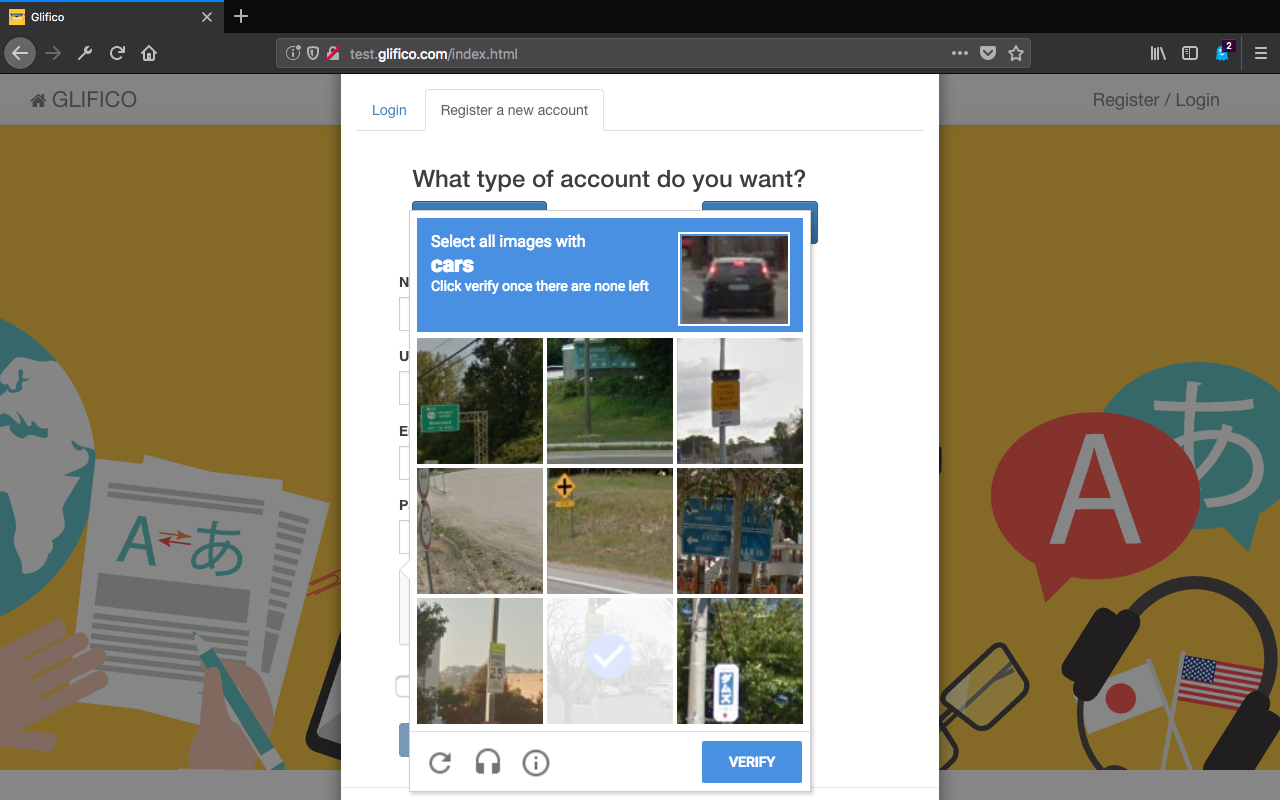
\includegraphics[width=0.95\textwidth]{register_translator4.png}
\end{figure}

\begin{figure}[H]
\centering
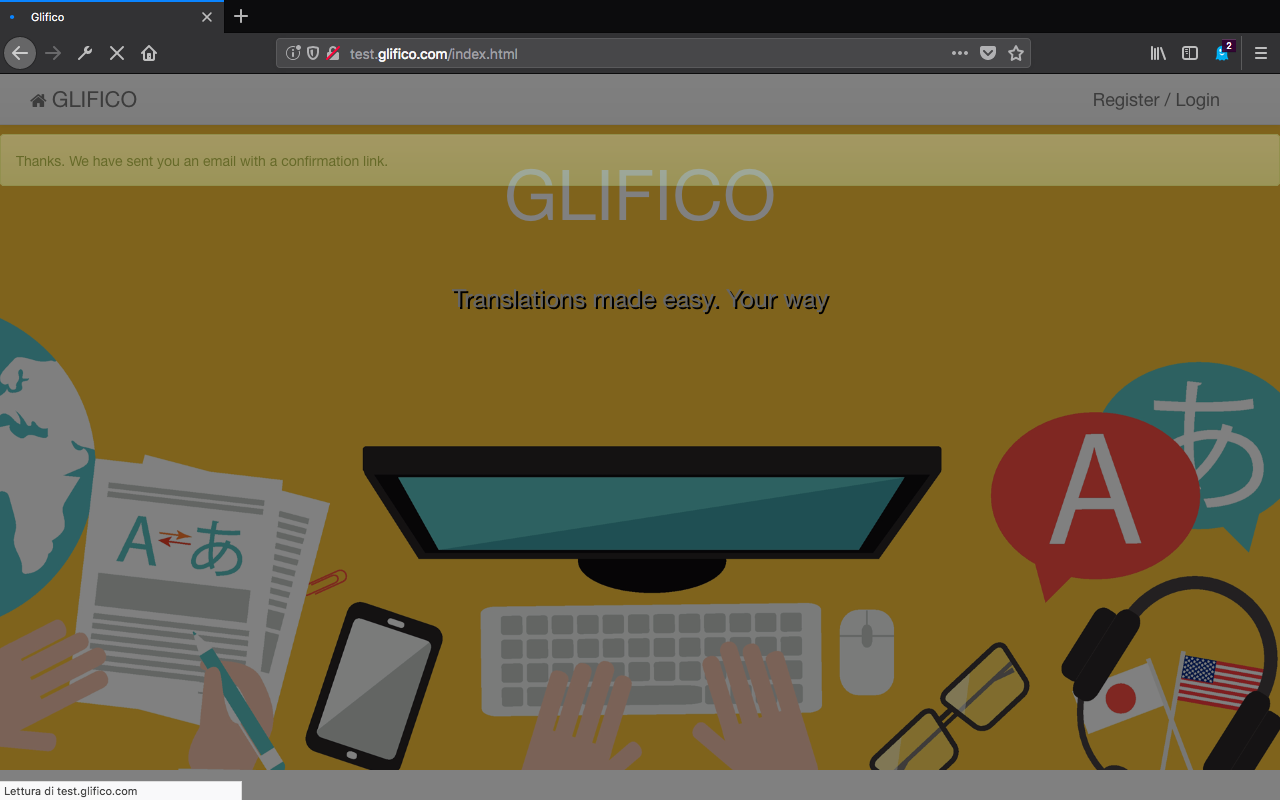
\includegraphics[width=0.95\textwidth]{register_translator5.png}
\end{figure}

\clearpage
Go to your email (this window depends on your email provider) and click the link
\begin{figure}[H]
\centering
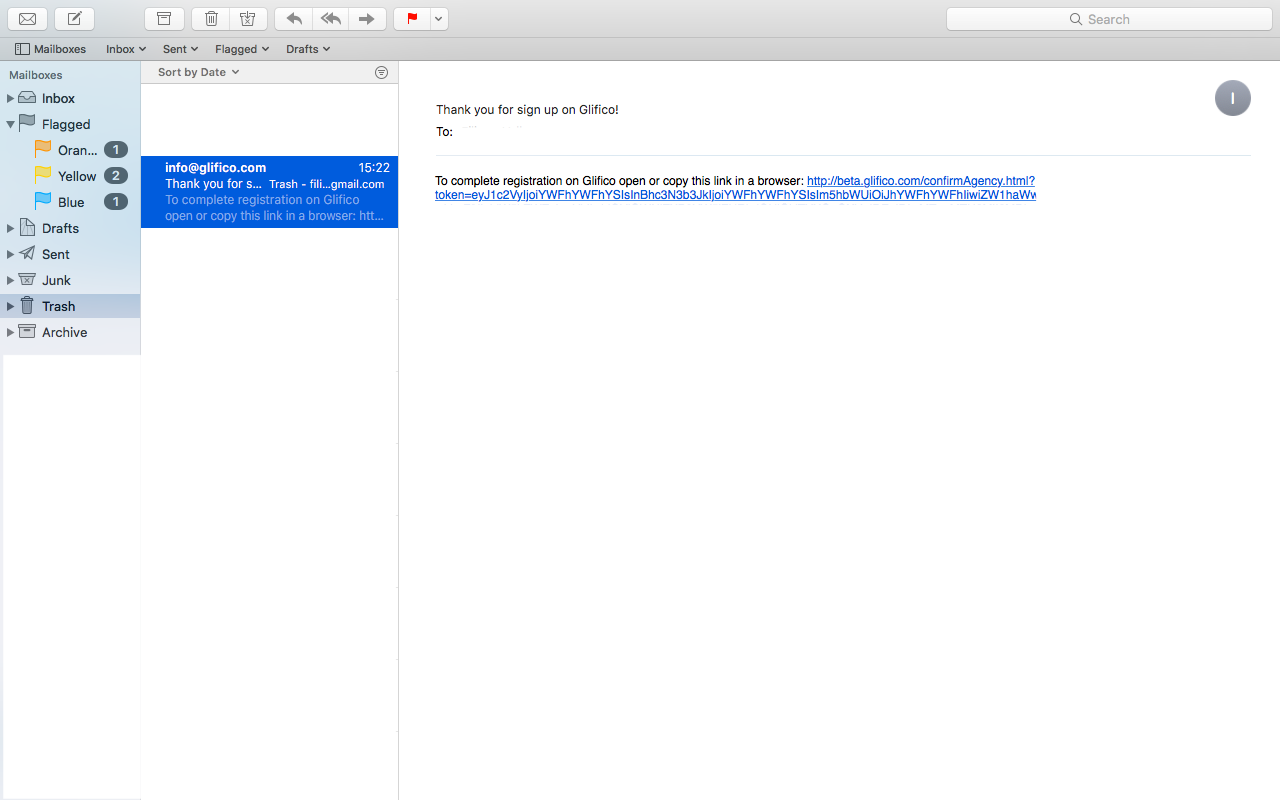
\includegraphics[width=0.95\textwidth]{register_translator6.png}
\end{figure}

You're redirect on a welcome page
\begin{figure}[H]
\centering
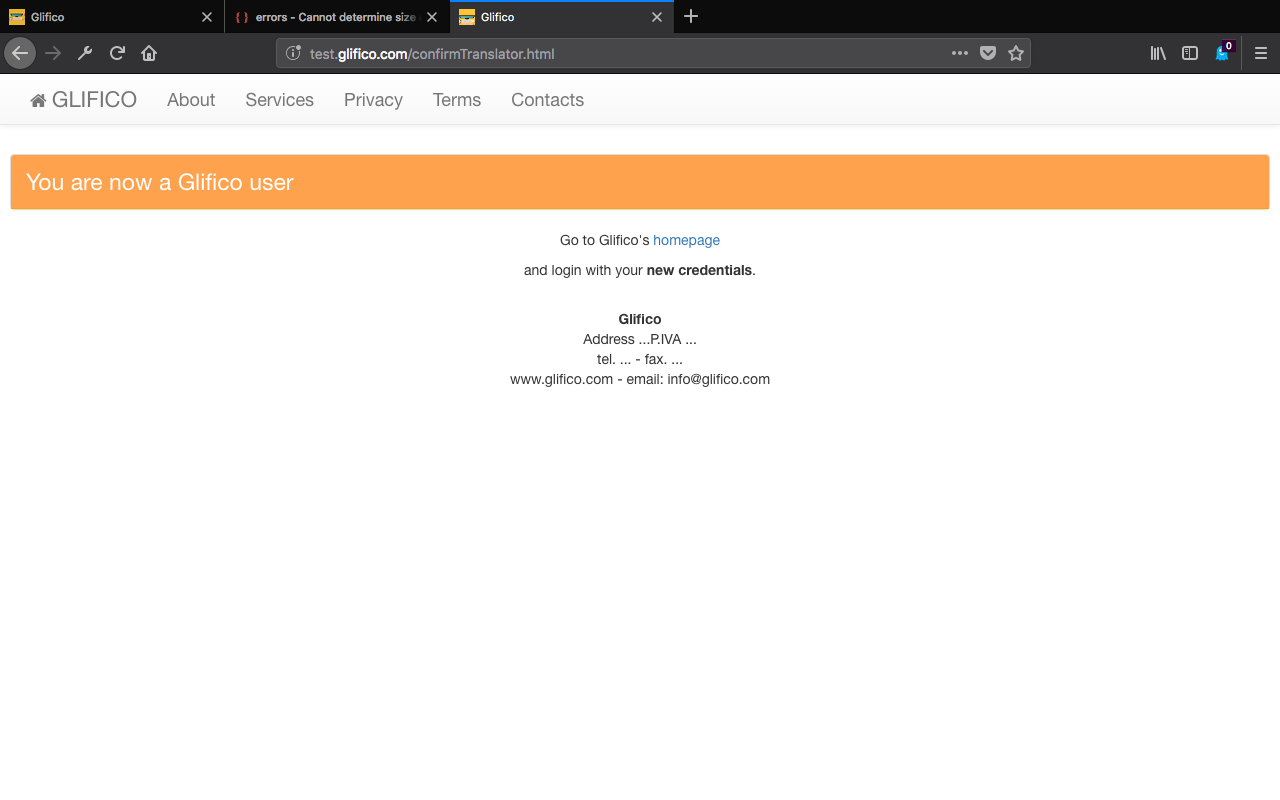
\includegraphics[width=0.95\textwidth]{register_translator7.png}
\end{figure}

\clearpage
Go to homepage and login
\begin{figure}[H]
\centering
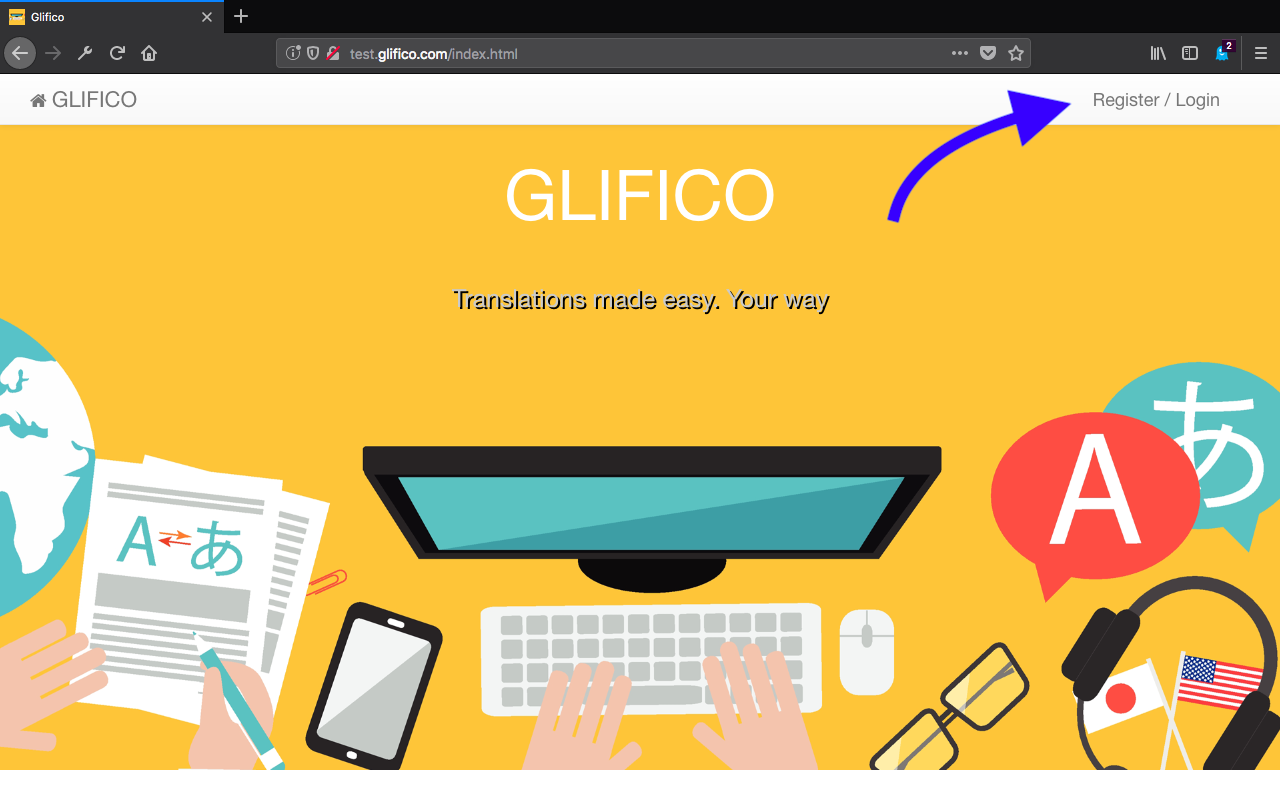
\includegraphics[width=0.95\textwidth]{register_translator0.png}
\end{figure}

Use your new credentials
\begin{figure}[H]
\centering
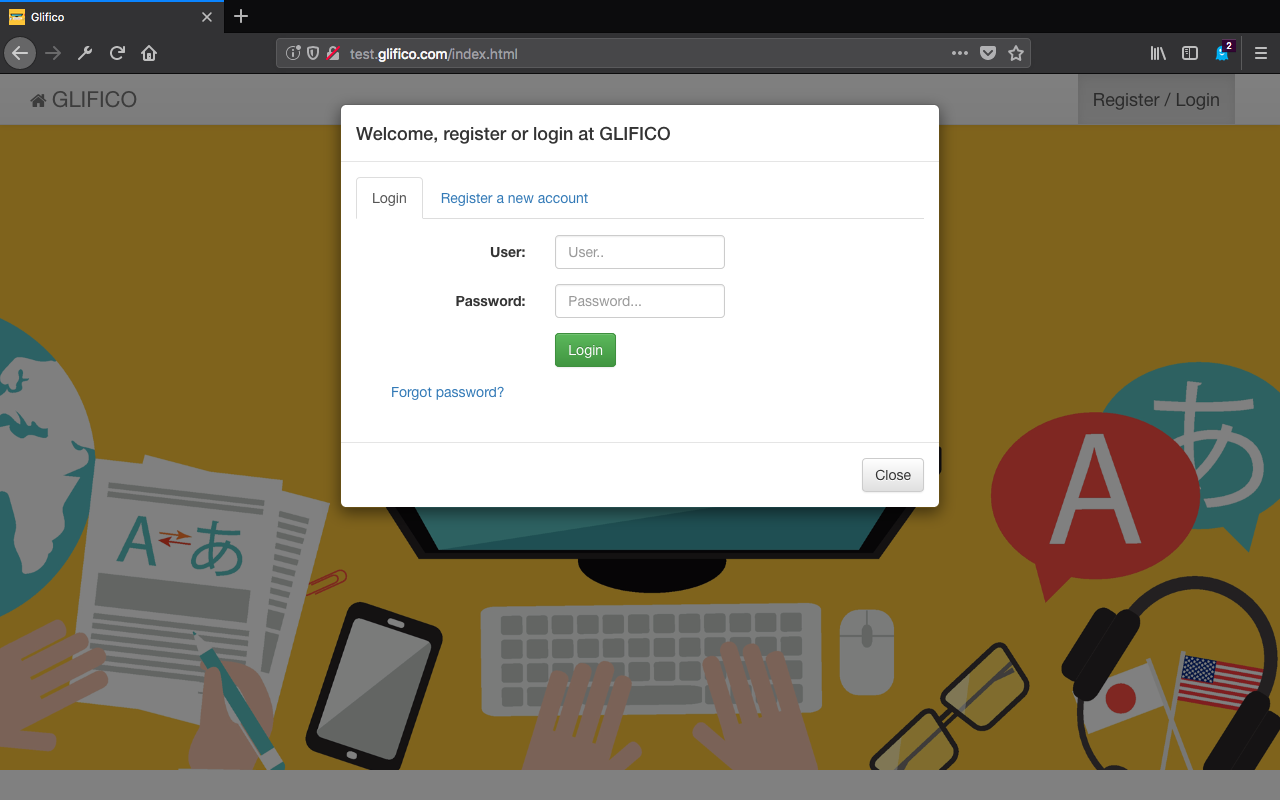
\includegraphics[width=0.95\textwidth]{login.png}
\end{figure}

\clearpage
\section{Fill your information}


\clearpage
\section{Add languages}
Follow this step to tell Glifico in which languages you are able to translate.

If not already there, go to your personal page
\begin{figure}[H]
\centering
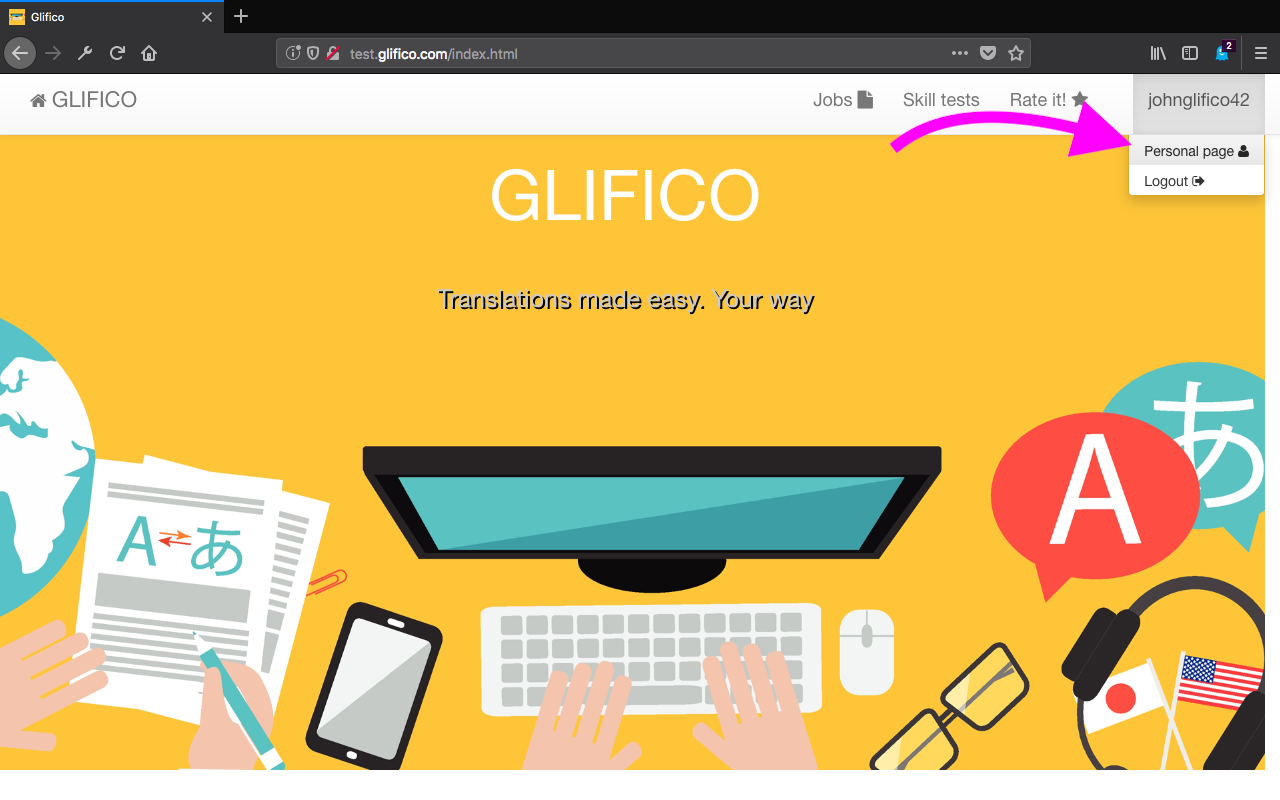
\includegraphics[width=0.95\textwidth]{translator_pair0.png}
\end{figure}

Select \textit{Your Languages}
\begin{figure}[H]
\centering
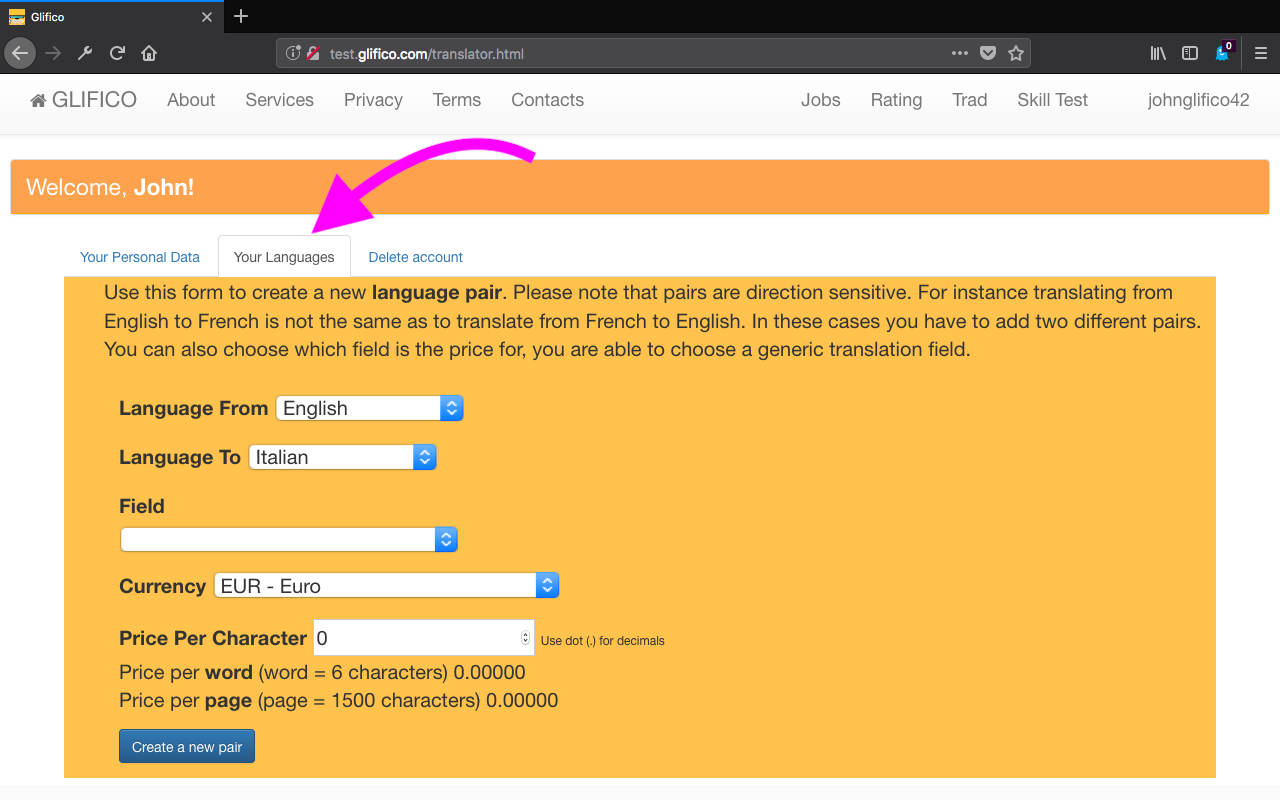
\includegraphics[width=0.95\textwidth]{translator_pair1.png}
\end{figure}


\clearpage
Fill information, choose a field 
\begin{figure}[H]
\centering
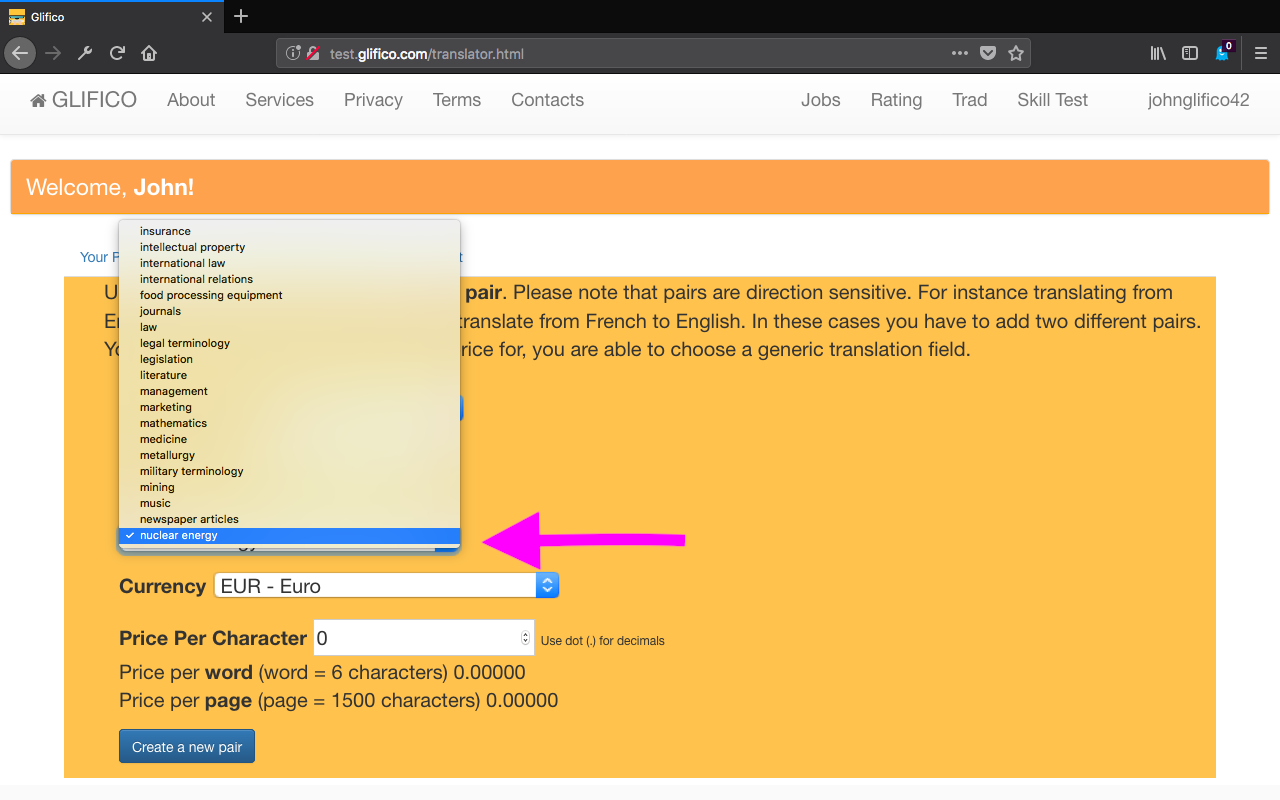
\includegraphics[width=0.95\textwidth]{translator_pair2.png}
\end{figure}

Chose the currency
\begin{figure}[H]
\centering
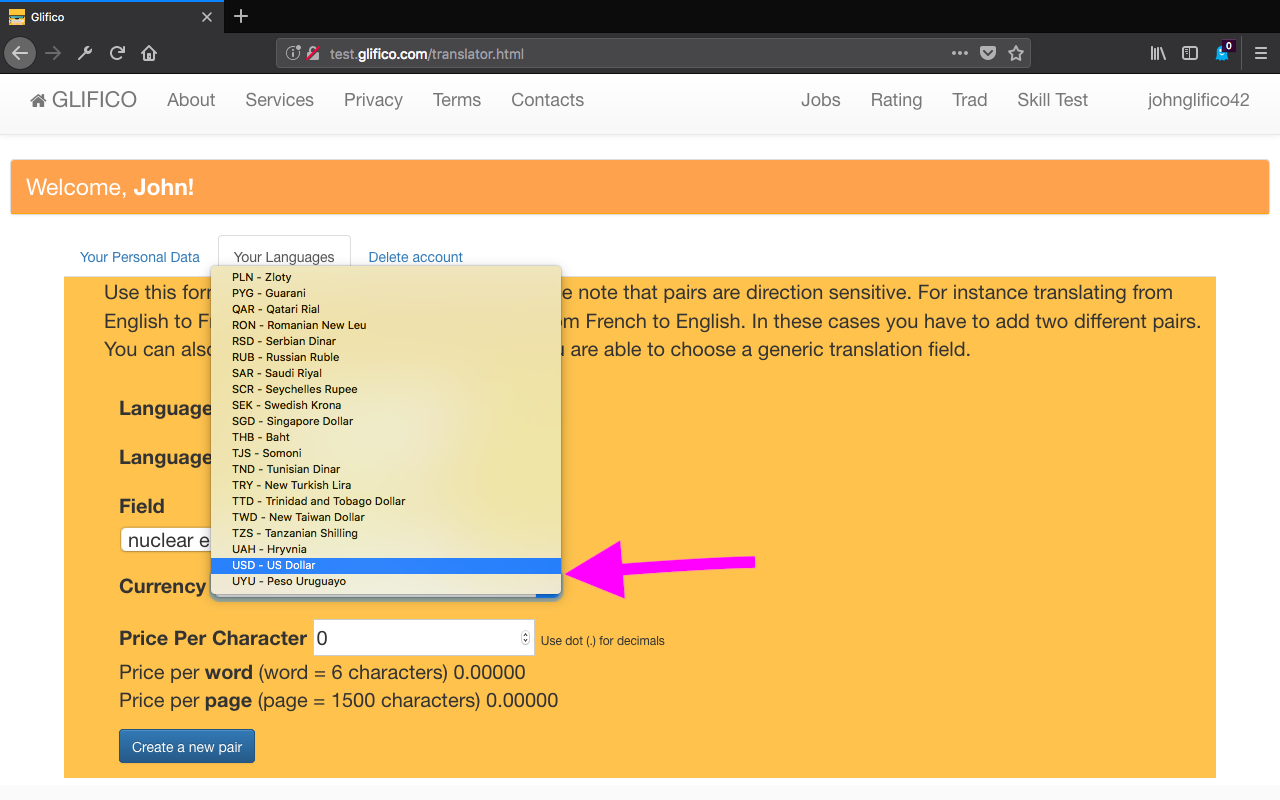
\includegraphics[width=0.95\textwidth]{translator_pair3.png}
\end{figure}

Insert the price per character (use "." for decimals) and check the price per word and per page.


\clearpage
Click \textit{Update my data} and wait confirmation from the server
\begin{figure}[H]
\centering
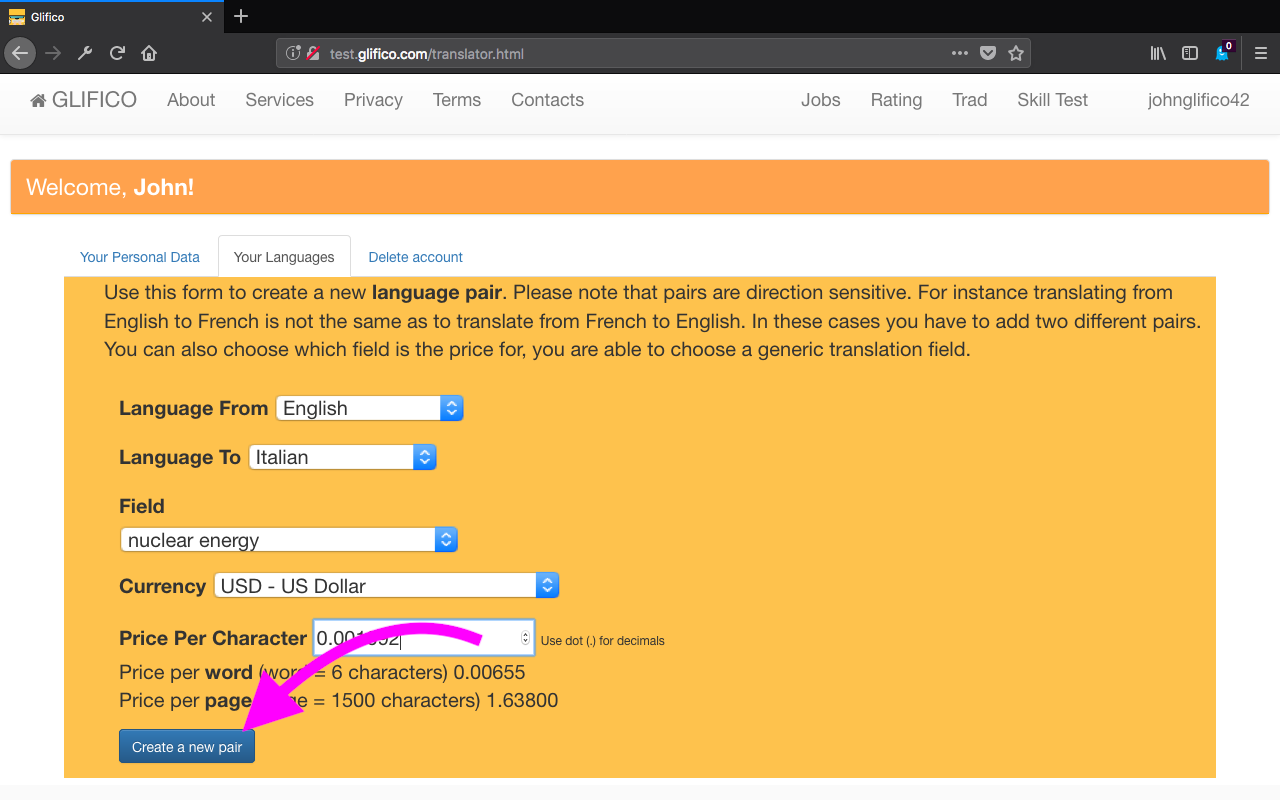
\includegraphics[width=0.95\textwidth]{translator_pair4.png}
\end{figure}


\begin{figure}[H]
\centering
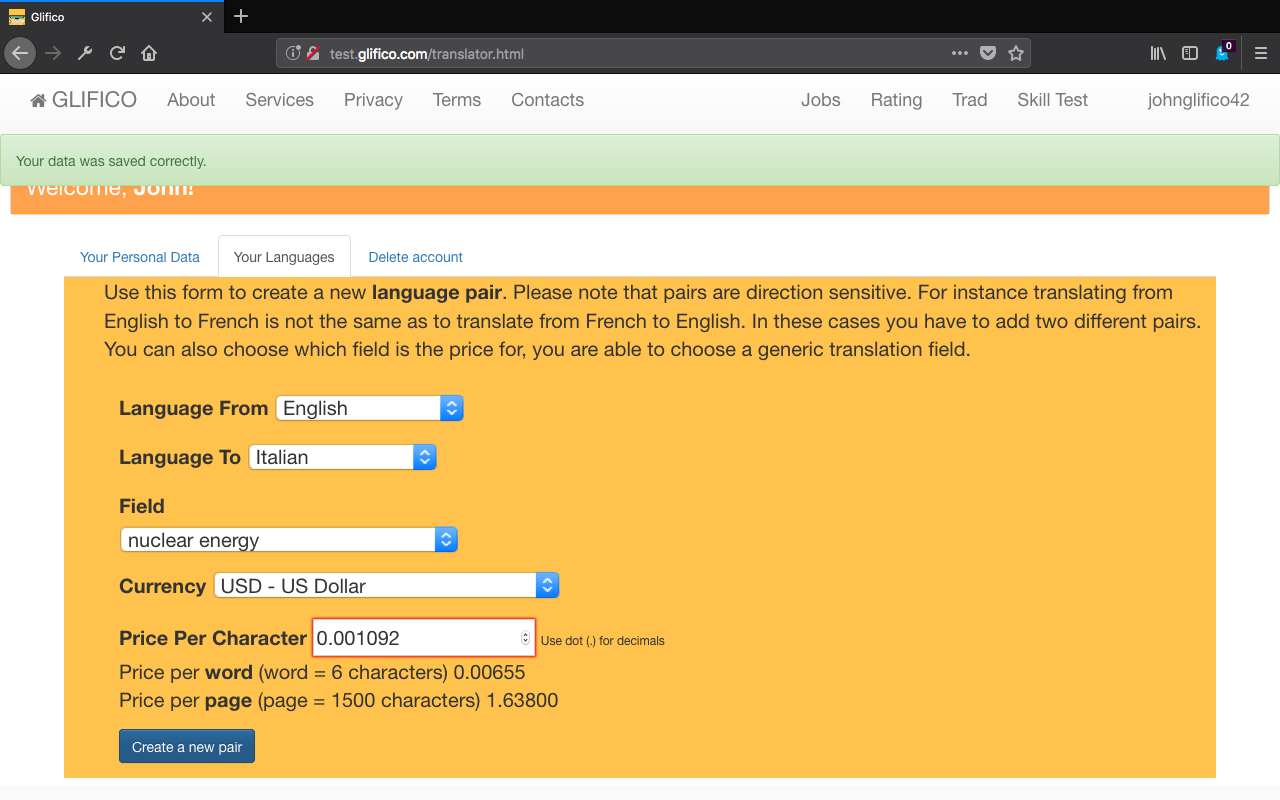
\includegraphics[width=0.95\textwidth]{translator_pair5.png}
\end{figure}


\clearpage
Look your new pair
\begin{figure}[H]
\centering
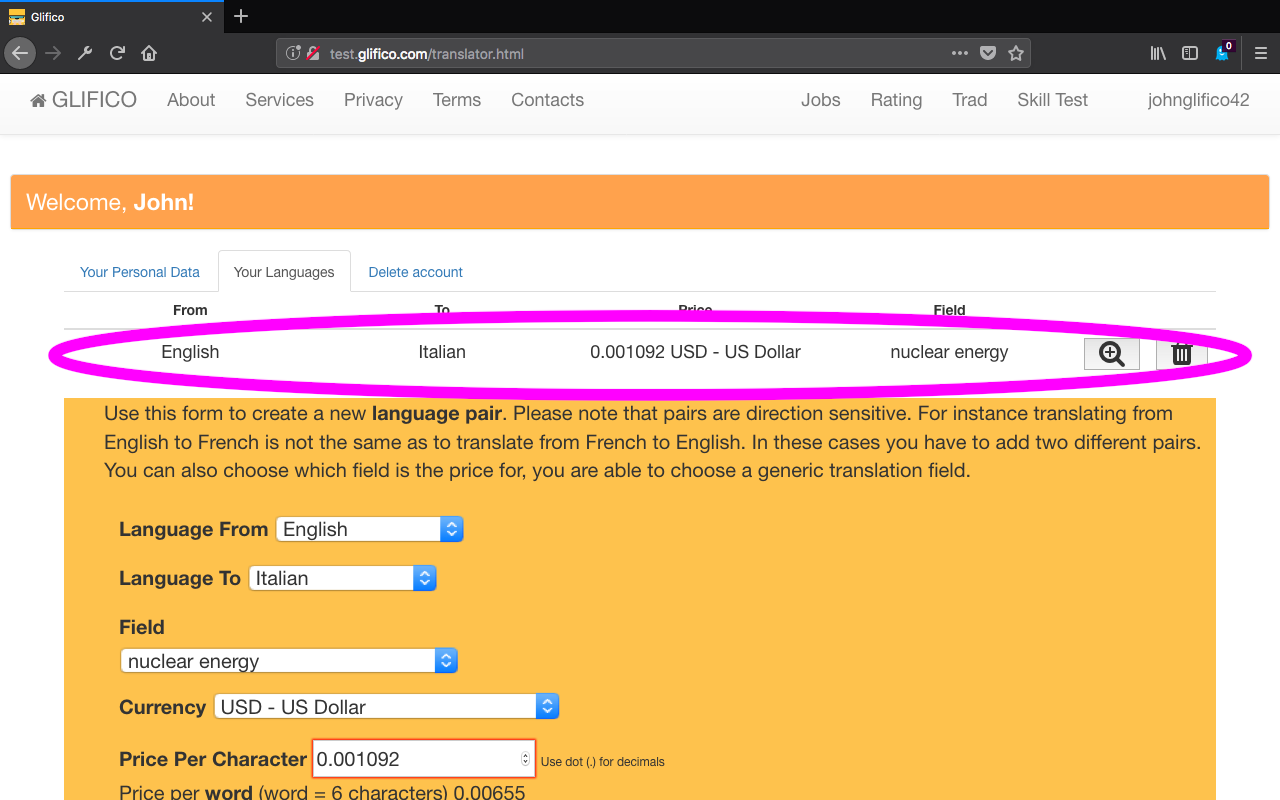
\includegraphics[width=0.95\textwidth]{translator_pair6.png}
\end{figure}

Click the magnifier icon to see details
\begin{figure}[H]
\centering
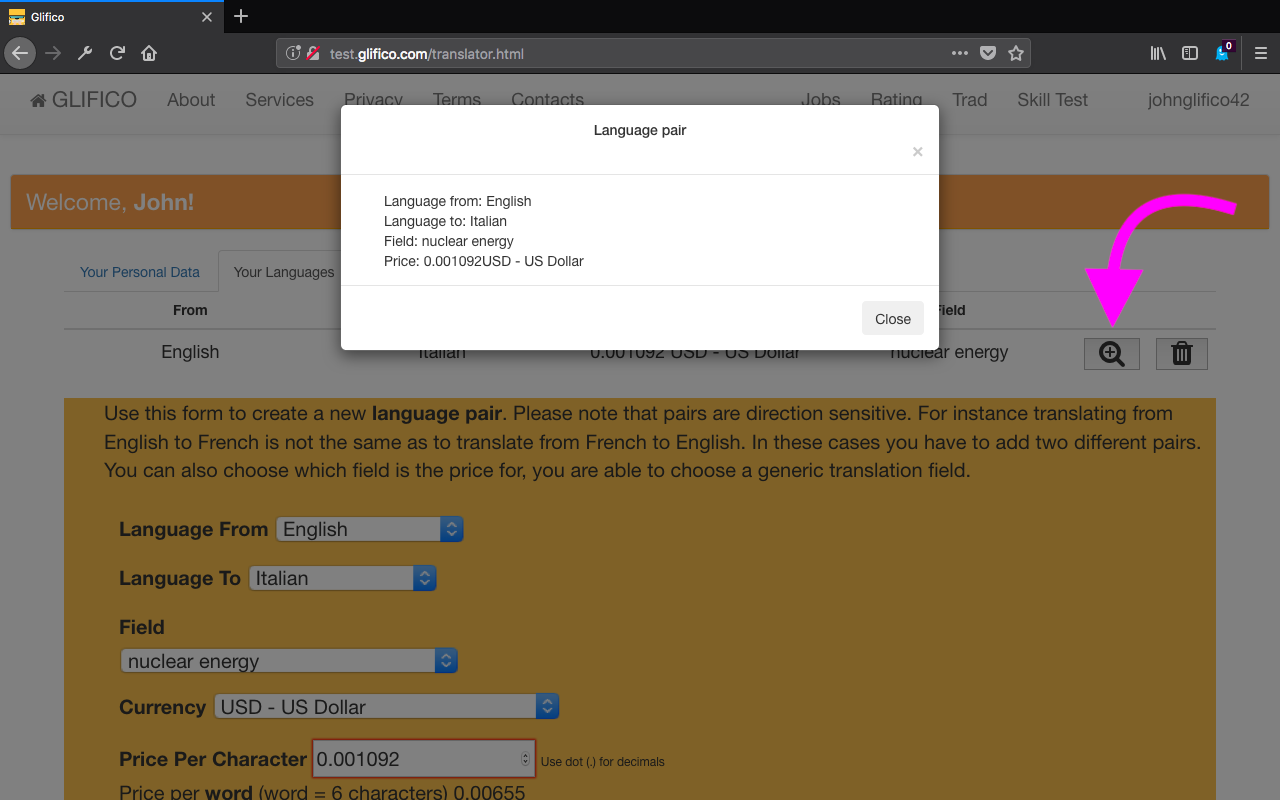
\includegraphics[width=0.95\textwidth]{translator_pair7.png}
\end{figure}


\clearpage
\subsection{Delete a language pair}
To remove a pair simply click the bin icon
\begin{figure}[H]
\centering
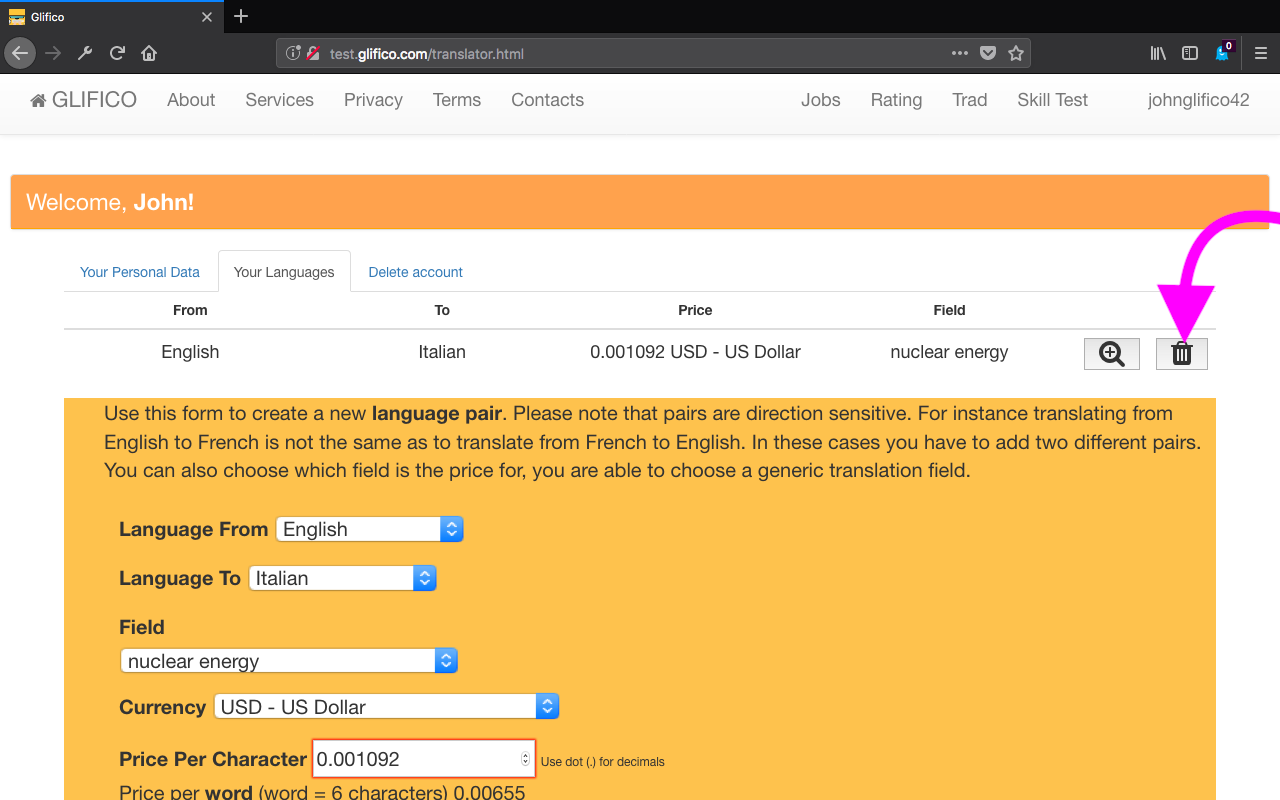
\includegraphics[width=0.95\textwidth]{translator_pair8.png}
\end{figure}

Glifico will not remove a language pair if you're working on jobs in that languages.

\clearpage
\section{A job on Glifico}
Follow this steps to accept, translate and complete a job.
First of all go to jobs' page
\begin{figure}[H]
\centering
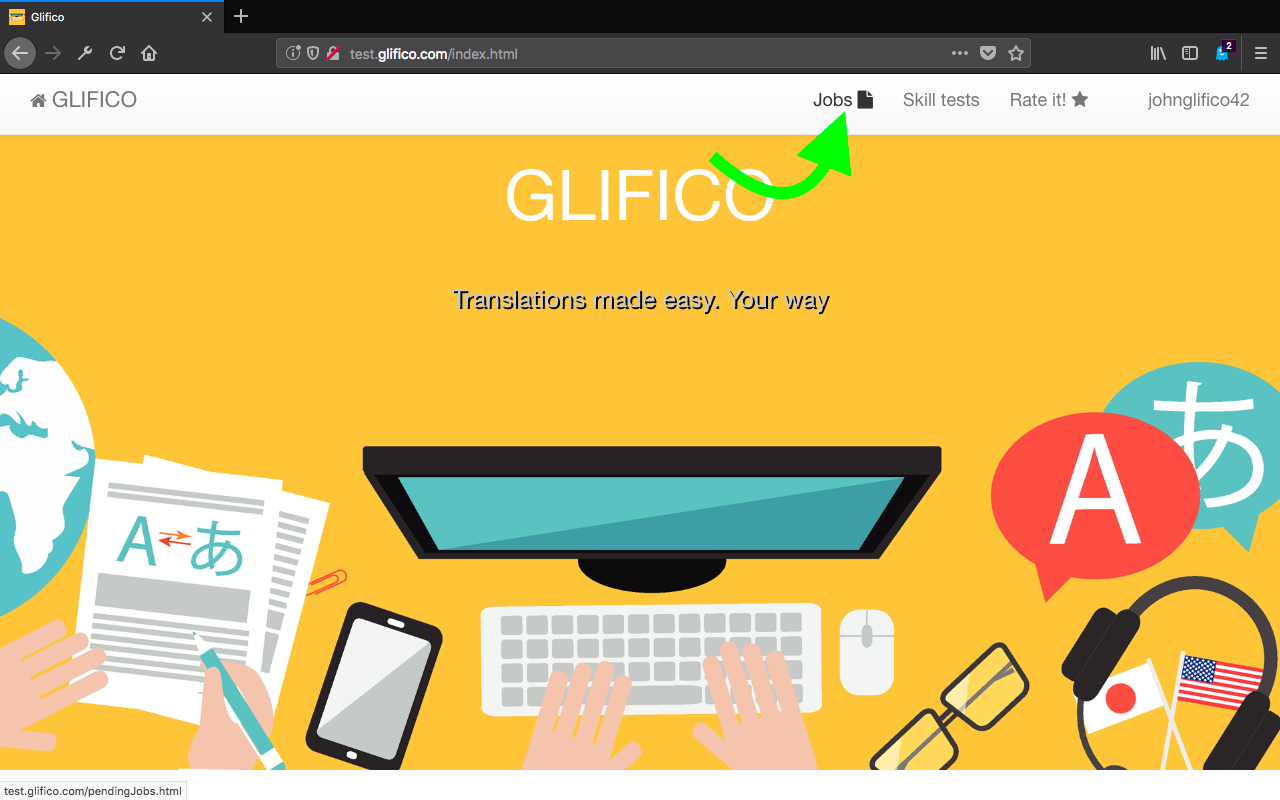
\includegraphics[width=0.9\textwidth]{translator_job0.png}
\end{figure}

Here you can see all your jobs, in particular the one \textit{To Be Assigned}, click \textit{Show Job} for more information
\begin{figure}[H]
\centering
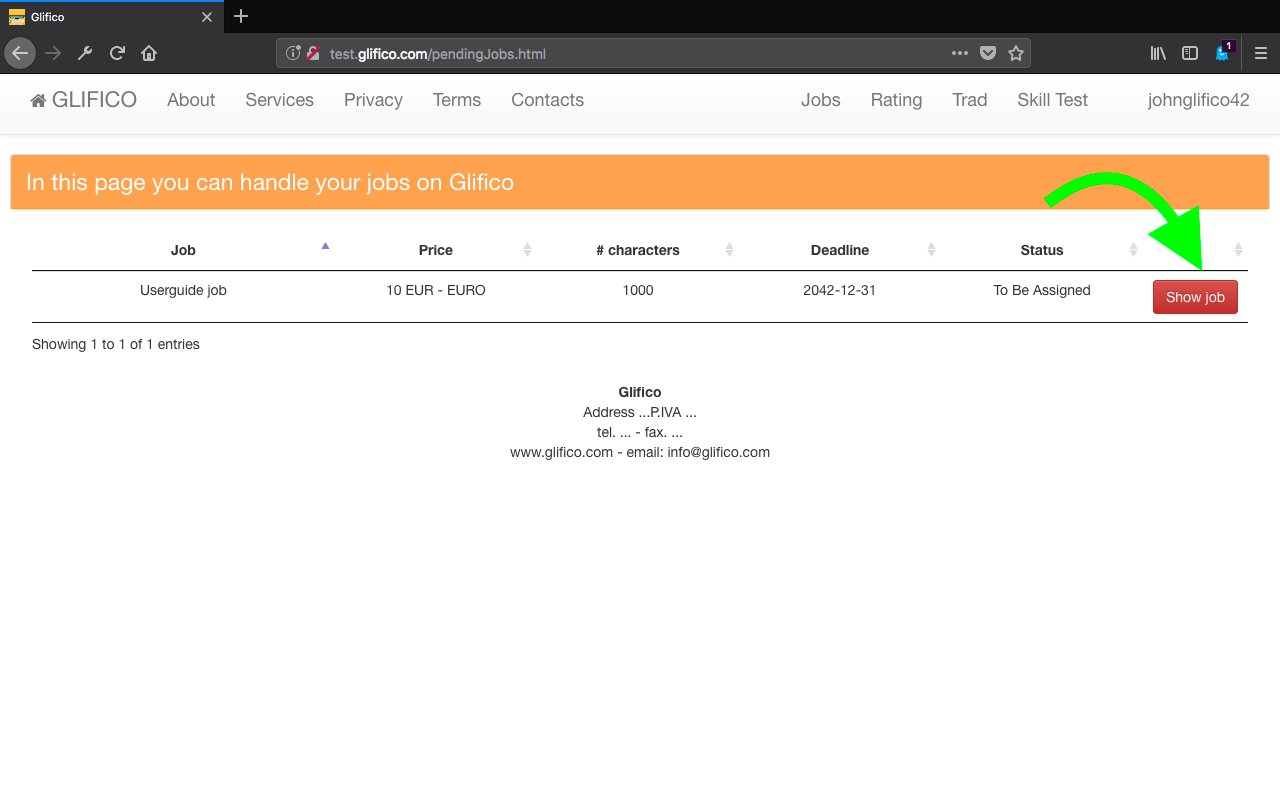
\includegraphics[width=0.85\textwidth]{translator_job1.png}
\end{figure}


\clearpage
Here you can see the job proposed by the agency in details
\begin{figure}[H]
\centering
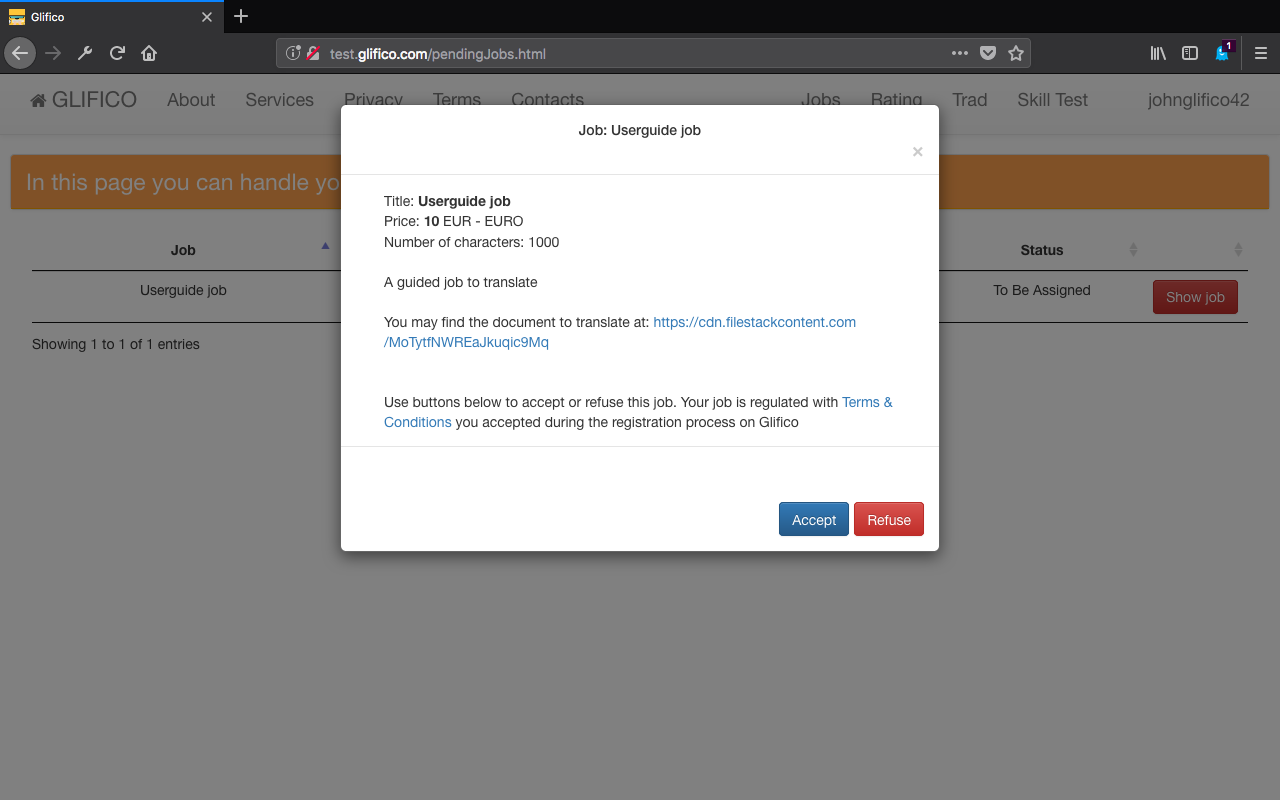
\includegraphics[width=0.95\textwidth]{translator_job2.png}
\end{figure}

Click \textit{Accept} if you are going to get this job
\begin{figure}[H]
\centering
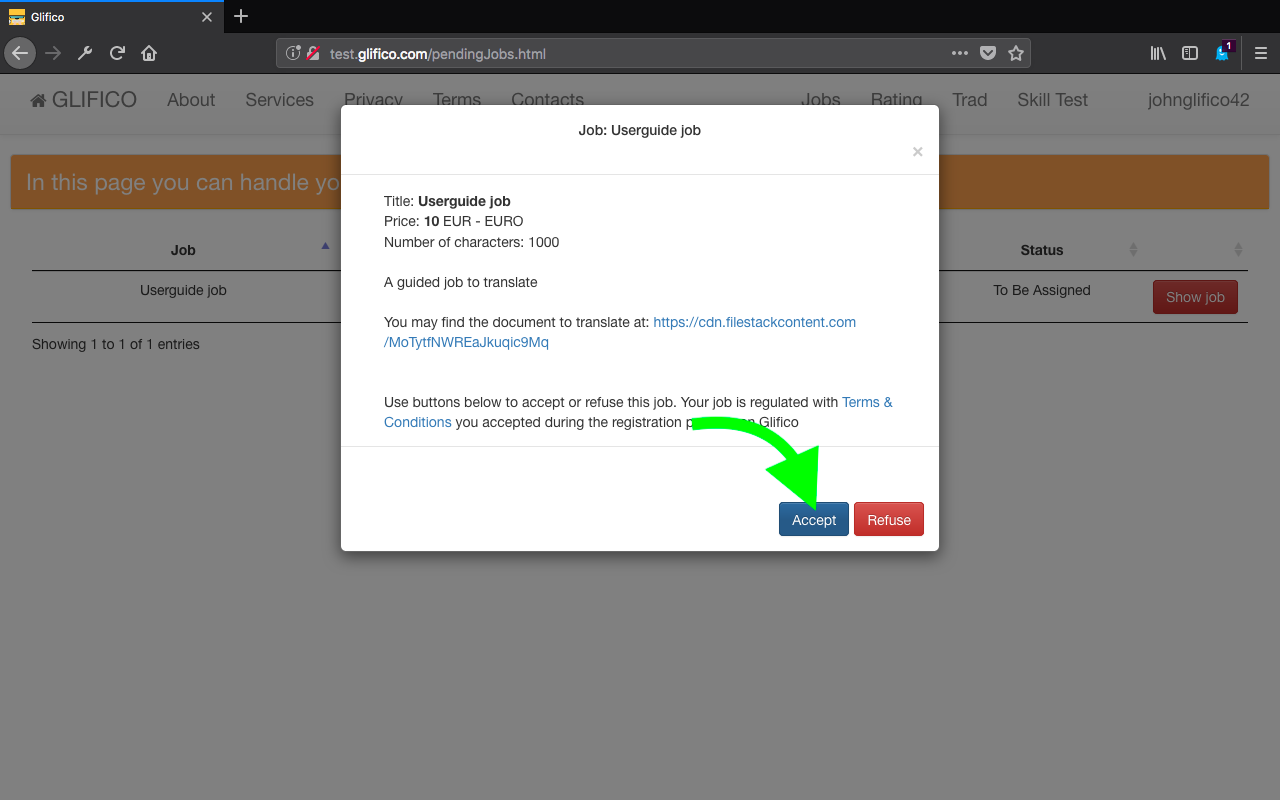
\includegraphics[width=0.95\textwidth]{translator_job3.png}
\end{figure}


\clearpage
If job is \textit{Accepted} you have time until the deadline to complete it...
\begin{figure}[H]
\centering
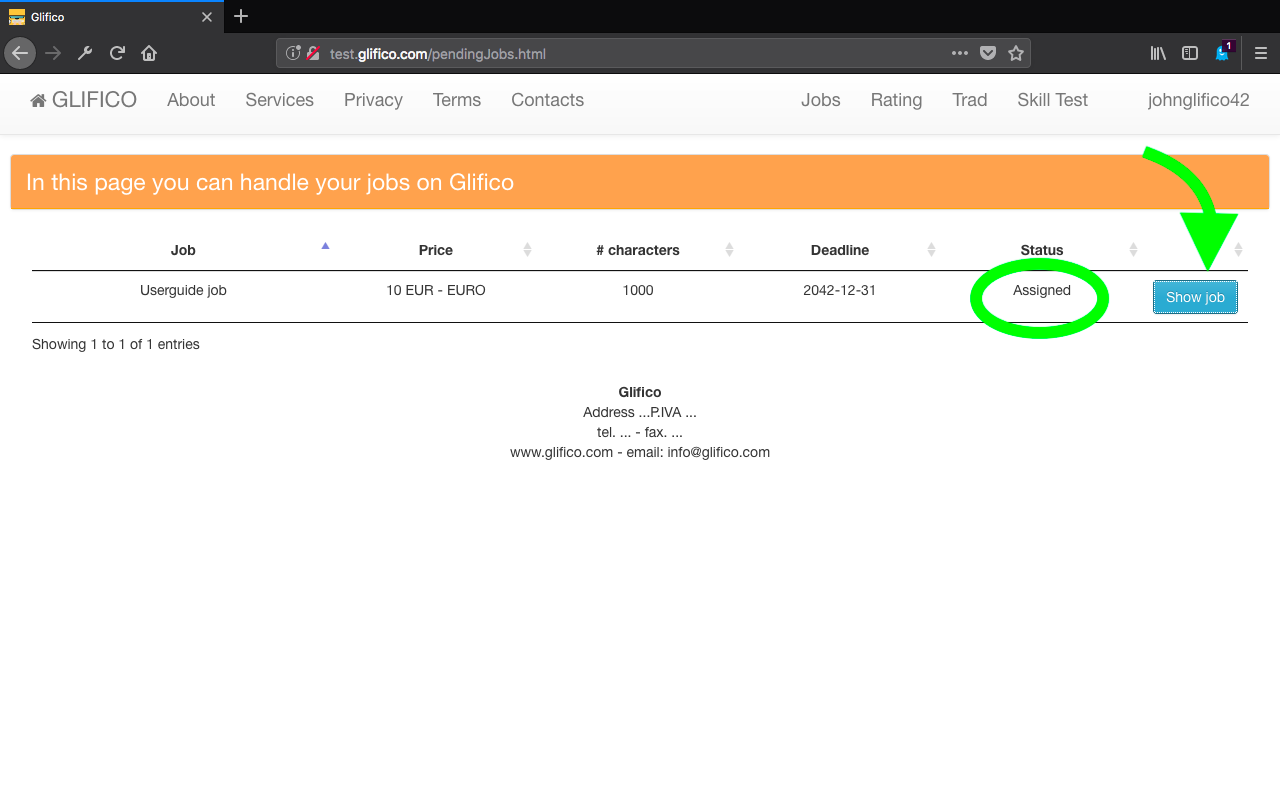
\includegraphics[width=0.95\textwidth]{translator_job4.png}
\end{figure}

...when you're done click \textit{Show Job} then you have to upload \textbf{two different documents}.
First of all upload a \textbf{preview} of your translation
\begin{figure}[H]
\centering
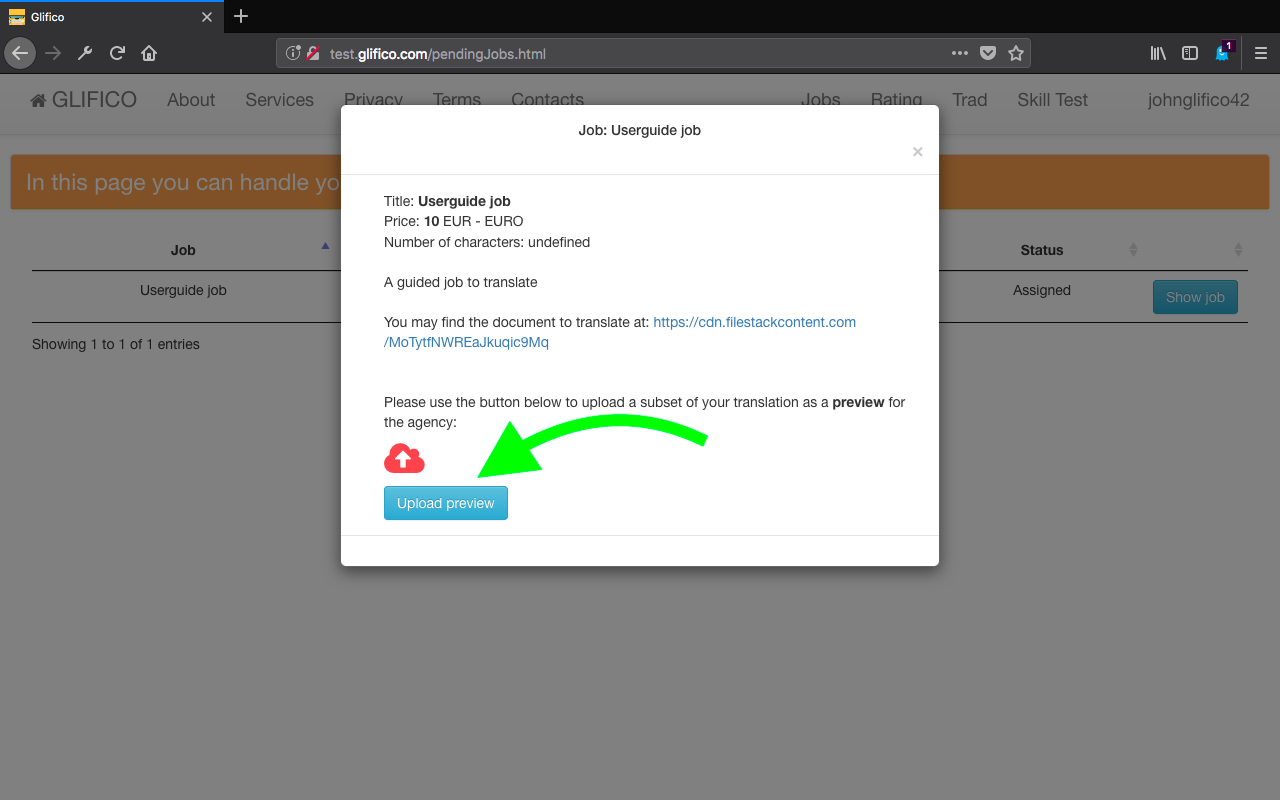
\includegraphics[width=0.95\textwidth]{translator_job5.png}
\end{figure}


\clearpage
Select file from your computer, Google Drive, Dropbox..
\begin{figure}[H]
\centering
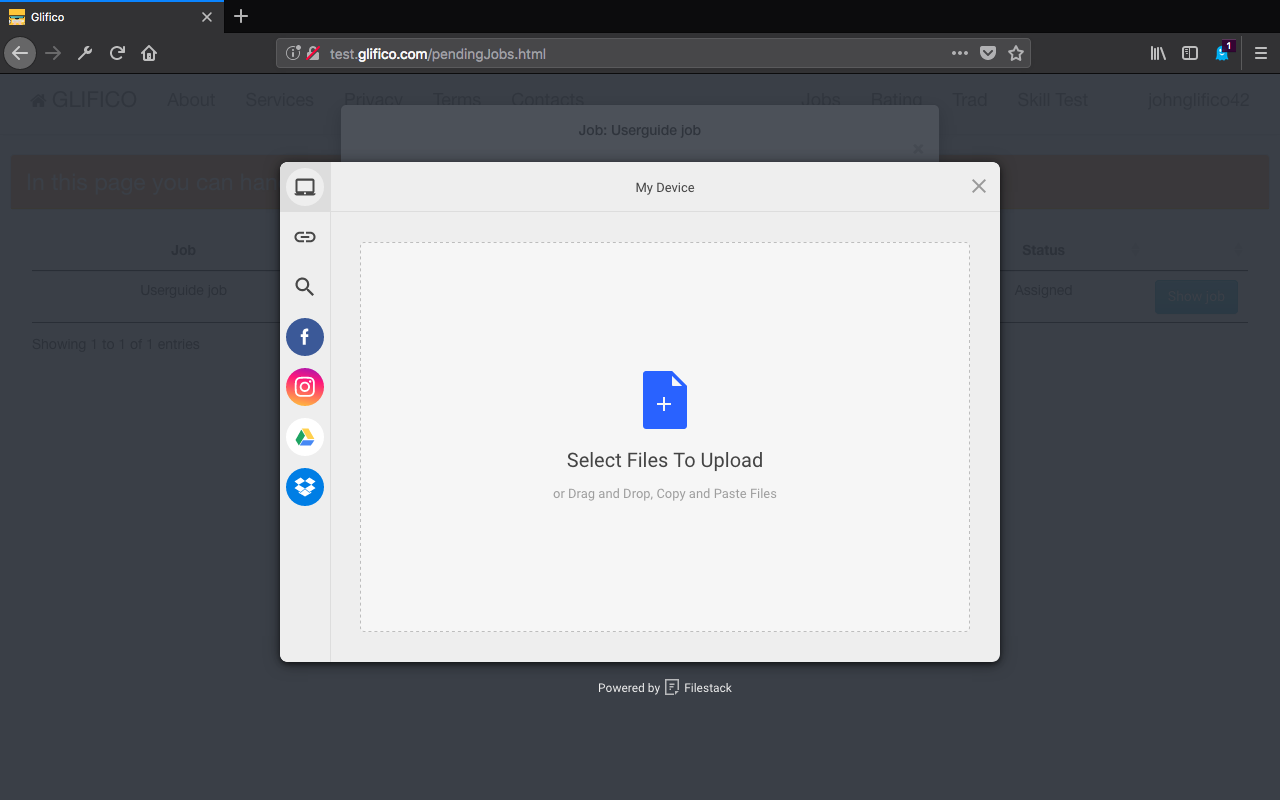
\includegraphics[width=0.95\textwidth]{translator_job6.png}
\end{figure}

Upload it
\begin{figure}[H]
\centering
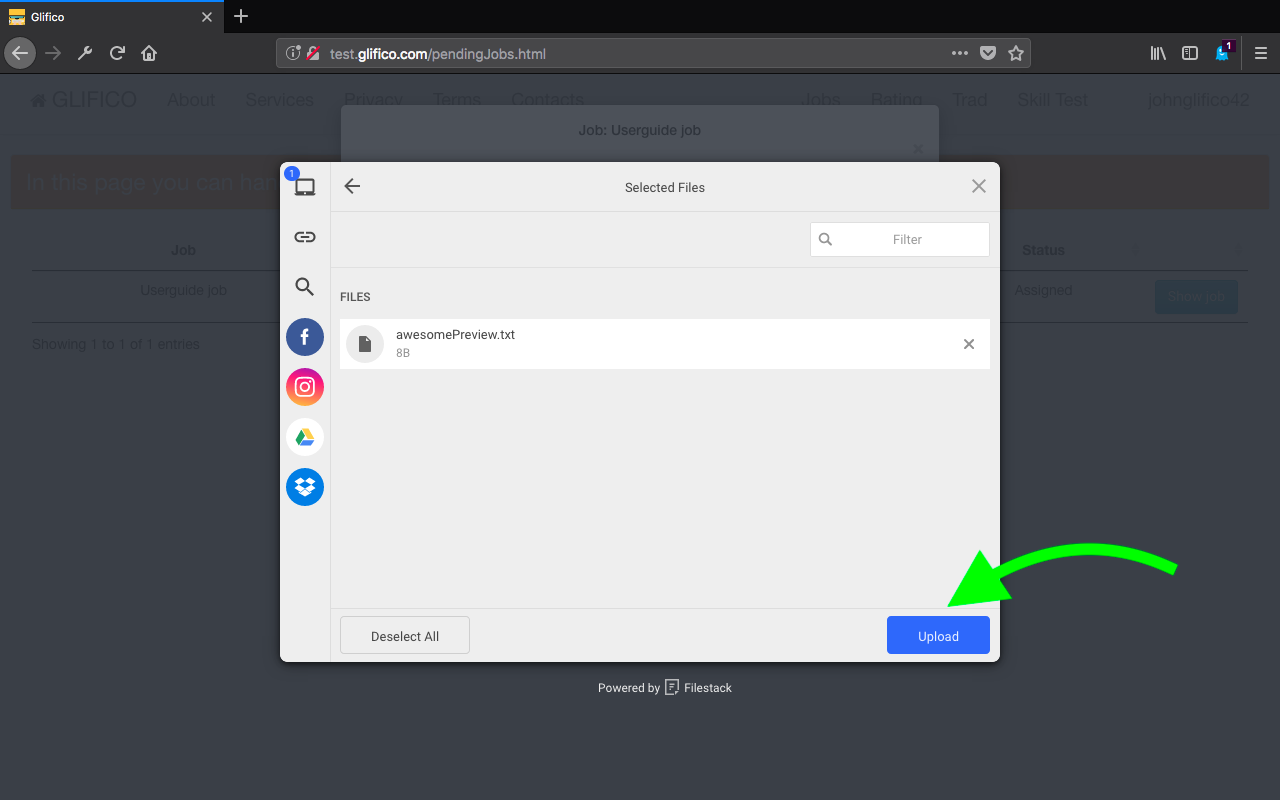
\includegraphics[width=0.95\textwidth]{translator_job7.png}
\end{figure}


\clearpage
Now you can upload the \textbf{full translated document}
\begin{figure}[H]
\centering
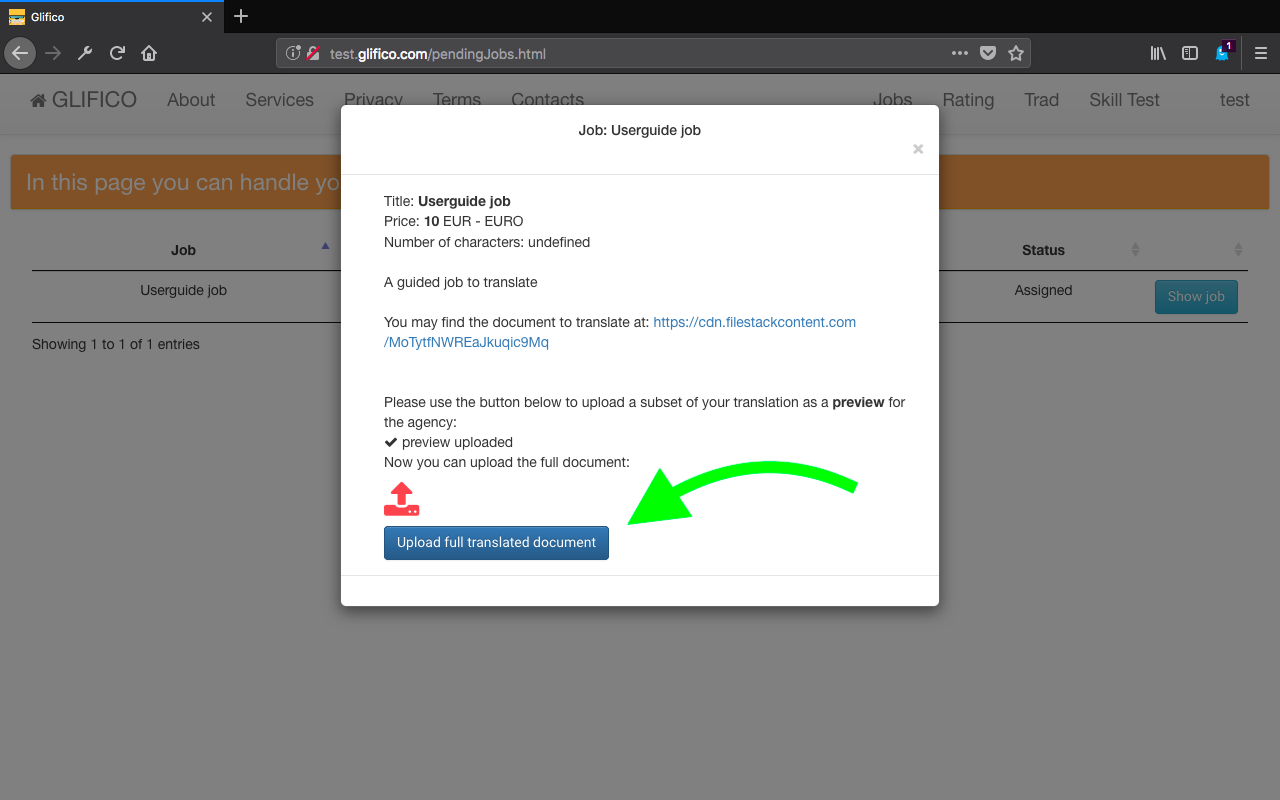
\includegraphics[width=0.95\textwidth]{translator_job8.png}
\end{figure}

Choose the file and upload it
\begin{figure}[H]
\centering
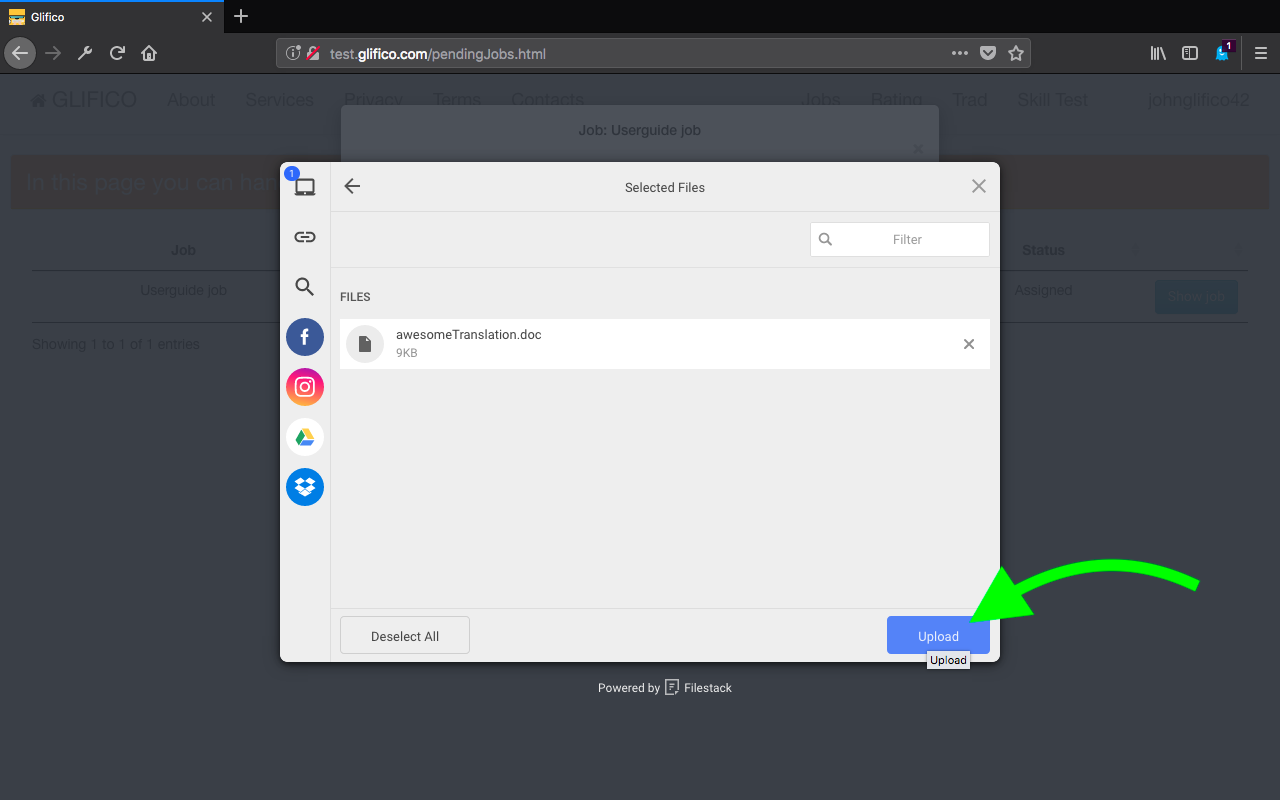
\includegraphics[width=0.95\textwidth]{translator_job9.png}
\end{figure}


\clearpage
Your job is now set as \textit{Translated}
\begin{figure}[H]
\centering
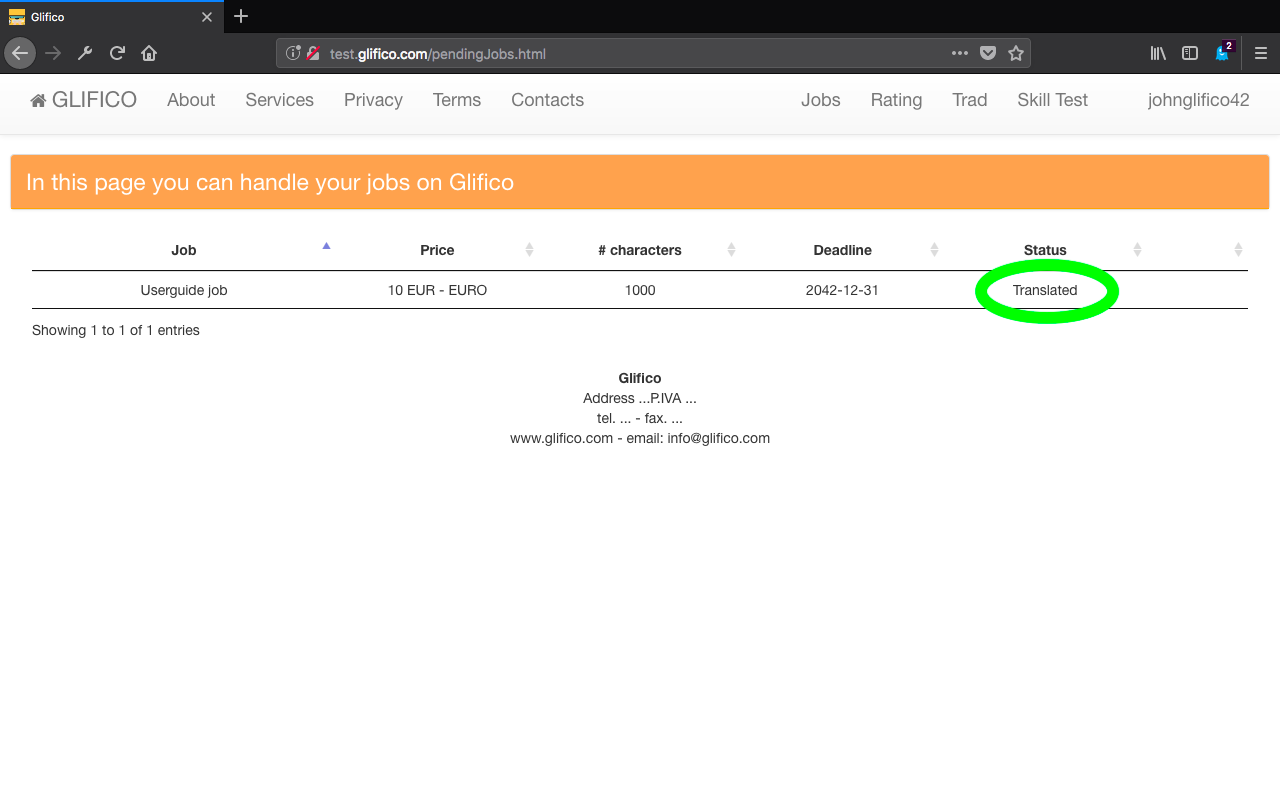
\includegraphics[width=0.95\textwidth]{translator_job10.png}
\end{figure}

Agency will evaluate your preview and eventually will accept the job
\begin{figure}[H]
\centering
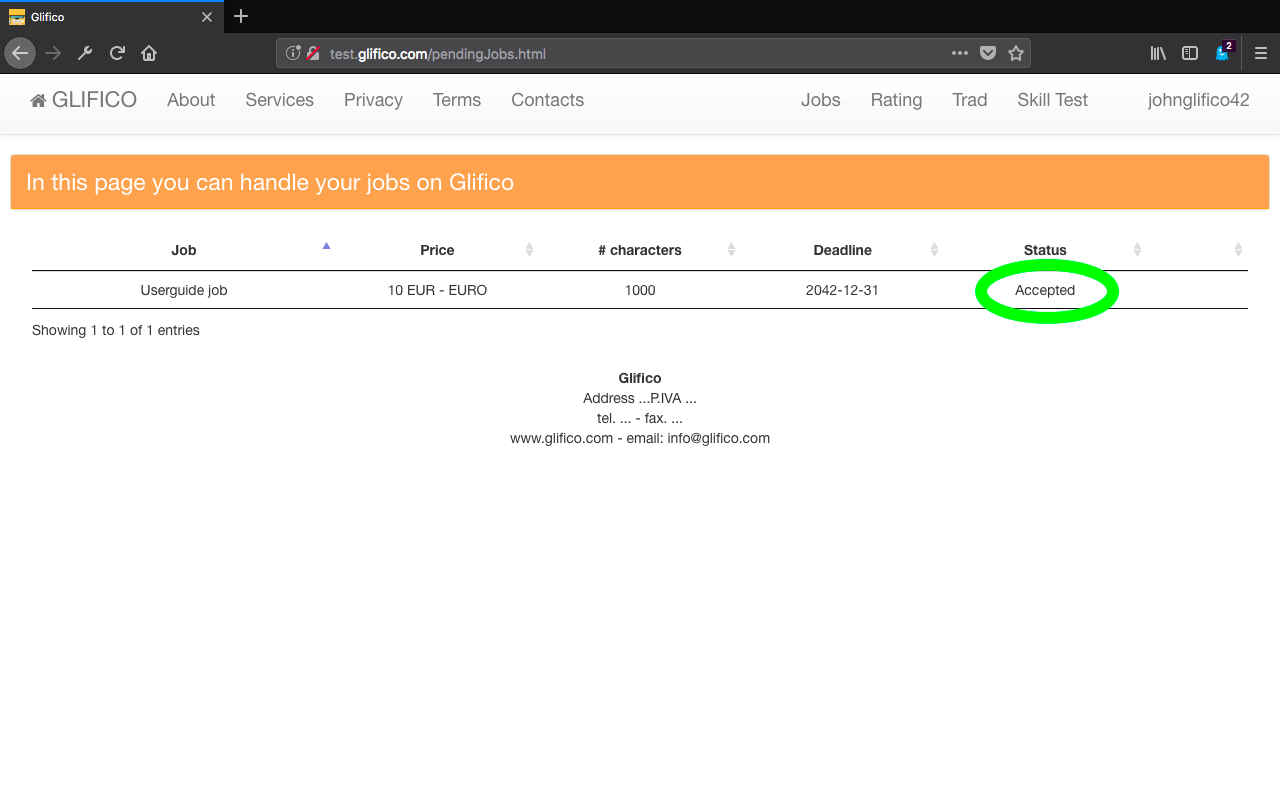
\includegraphics[width=0.95\textwidth]{translator_job11.png}
\end{figure}

\clearpage
Agency will pay the document set as \textit{Paid} and Glifico will pay you very soon..
\begin{figure}[H]
\centering
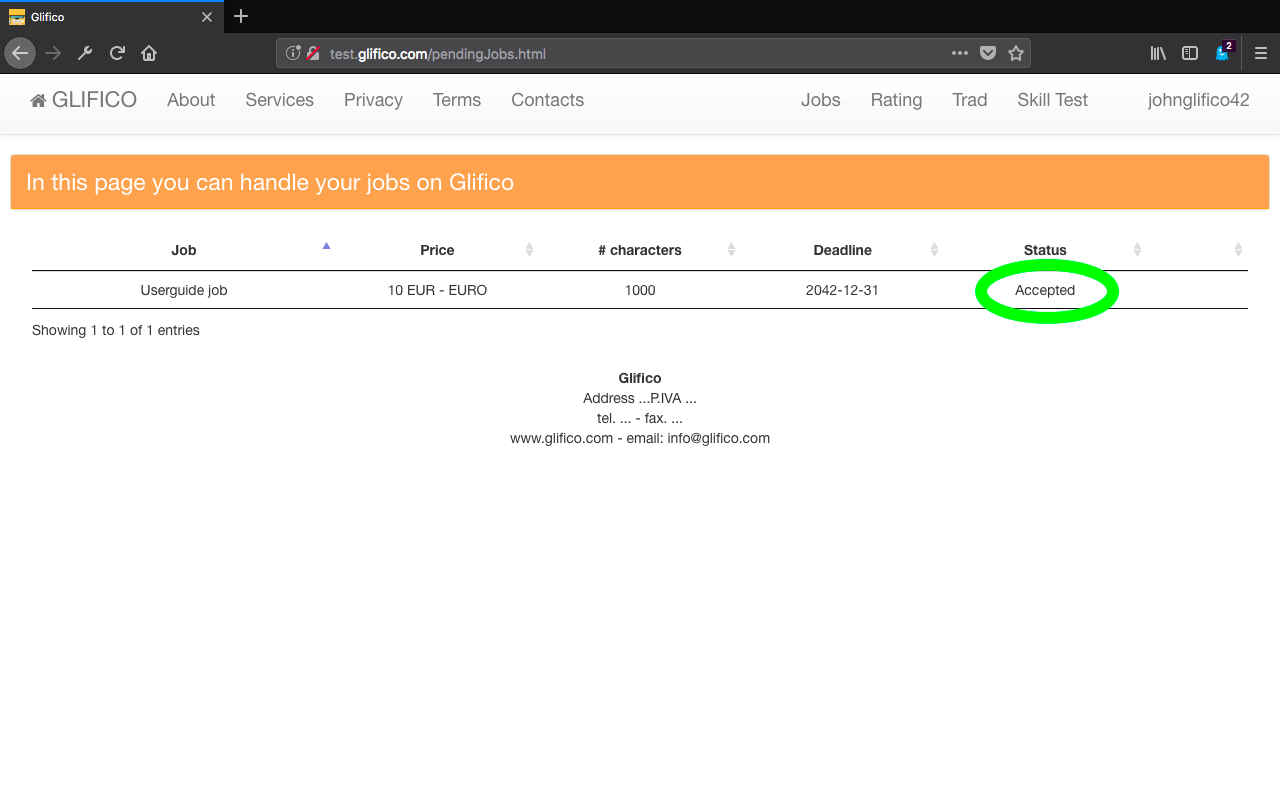
\includegraphics[width=0.95\textwidth]{translator_job11.png}
\end{figure}

\clearpage
\subsection{Refuse a job}
When a job is proposed to you, simply click \textit{Refuse} to ignore the job
\begin{figure}[H]
\centering
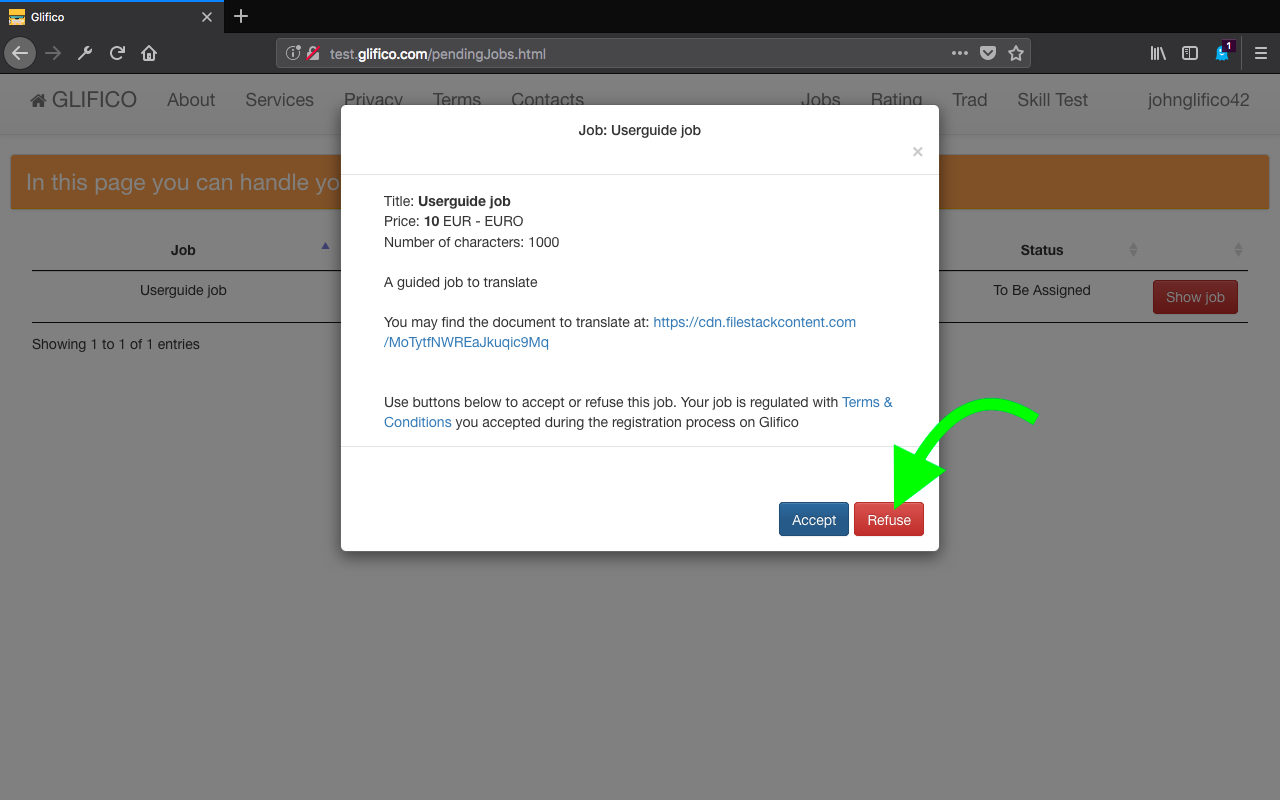
\includegraphics[width=0.95\textwidth]{translator_job3_del.png}
\end{figure}

\clearpage
\section{Help}
Need help with anything?

Send an email to \href{mailto:info@glifico.com}{\nolinkurl{info@glifico.com}}

\end{document}
